\cleardoublepage

\chapter{Proposed Approach}
\label{ch:initial_work}

This chapter aims at making clear how the automatic image retrieval system was built and how it operates.



Initially in Section \ref{sec:diagram} the system workflow architecture is illustrated trough a diagram and a small description is present. Section \ref{sec:testruns} describes some of the preliminary experiences done to image recognition algorithms and object detection models provided by the ImageAI library in order to find the best performers. After, Section \ref{sec:alpha_retrieval} describes a very raw first attempt at an image retrieval system using only object detection. The implementation of the scene recognition algorithm is demonstrated in Section \ref{sec:scene_recognition}. Following up, in Section \ref{sec:runs} a description of the differences in the image processing stage between the submitted runs for the challenges is presented. Then, the text processing stage is introduced in Section \ref{sec:text}, in this section there is an explanation to how the system was able to extract linguistic annotations, what kind of syntax and semantic rules were implemented in the algorithm and how the categorization and extraction of relevant words from text was done. Section \ref{sec:retrieval} explains how the system is capable of automatically retrieving images for a given moment described in text, how it is able to compare the similarity of the mined text words with the visual concept words and all the calculations it does in order to compute weights and scores. Lastly, Sections \ref{sec:run1} and \ref{sec:run2} explain both of the submitted runs for the automatic image retrieval system.



\section{System Workflow Architecture Diagram}
\label{sec:diagram}
   
\begin{figure}[H]
    \centering
    \captionsetup{justification=centering}
    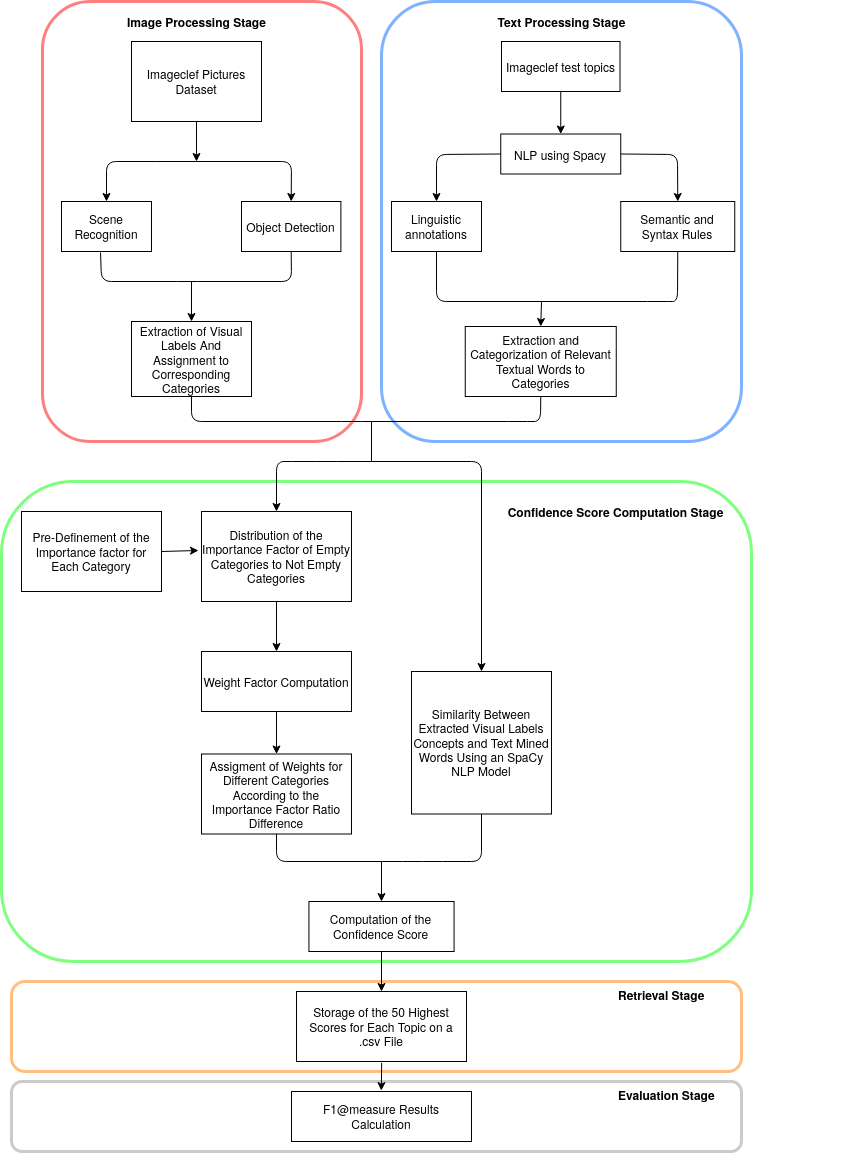
\includegraphics[width = 0.9\textwidth]{Sections/6textprocessing/images/diagram.png}
    \caption{System Architecture}
    \label{fig:testtopic}
  \end{figure}

\newpage

\begin{itemize}
  \item \textbf{Workflow Diagram Explained}
\end{itemize}

The system starts by firstly processing all images from the dataset provided by the imageCLEF challenge with scene and object recognition algorithms. During the process the labels are categorized according pre-defined categories.

Subsequently, text is processed using an NLP model that extracts linguistic annotations from textual sources.  With the implementation of syntax and semantic rules alongside with the provided linguistic annotations, relevant words are extracted and categorized in pre-defined categories. 

Following up, when all of the textual labels and visual labels are extracted and correctly categorized the confidence score computation stage starts. This stage has several steps that can be summarized in two main steps: the computation of weights for each category and the calculation of similarity scores.

Finally, in the retrieval stage, the system checks for the 50 highest confidence scores for a given topic and stores it in a csv file. This 50 images are the ones retrieved for a given moment.

As an extra step, an evaluation stage was created to analyse system results for the dev topics with the objective of emulating the evaluation methodology for the challenge.


  
  \section{Preliminary Experiences}
  \label{sec:testruns}

   With the goal of comparing the different image recognition algorithms and object detection models a few test runs were made. The models and algorithms were provided trough a computer vision python library called imageAI, which allows the ability to easily use state-of-the-art AI features. It supports algorithms for image prediction, custom image prediction, object detection, video detection, video object tracking and image predictions trainings \cite{ImageAI}.

  The test runs consist on feeding each of the models and algorithms with one picture manually chosen beforehand. Each model produces predictions on what the image represents or what the objected detected is. The prediction probability ranges in an interval between [0,100]. This prediction probability represents the certainty of the model or algorithm in the respective prediction.


  \par Sections \ref{sec:image_test} and \ref{sec:object_test} provide examples of the performance test runs done to the models and algorithms.

  \subsection{Image Recognition Preliminary Experiences}
  \label{sec:image_test}


  The imageAI library allows the usage of 4 image recognition algorithms for image recognition which are DenseNet, inceptionV3, ResNet50, and SquezeeNet. The experiences done to these algorithms consist in analysing one image and compare the results of the different algorithms with the goal of finding which one was the best performer and had the most accurate prediction with the highest prediction probability.
 
  In order to given a few examples of these preliminary experiences, the following 3 images in Figure \ref{fig:experi} were fully analysed with the image recognition algorithms.
\newpage
\begin{itemize}
  \item \textbf{Picture samples for image recognition tests}
\end{itemize}

  \begin{figure}[H]
    \centering
    \captionsetup{justification=centering}
  
    \begin{subfigure}{0.35\textwidth}
    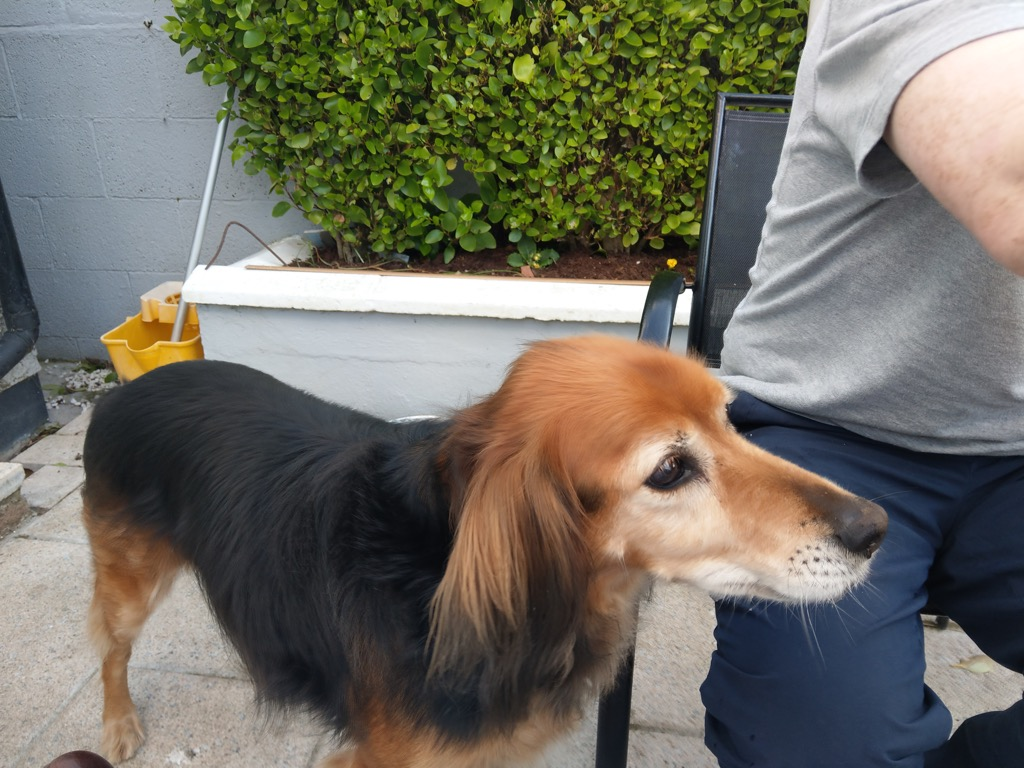
\includegraphics[width=\textwidth]{Sections/4InitialWork/4_images/run1_pic.jpg}
    \caption{} 
    \end{subfigure}
    \begin{subfigure}{0.35\textwidth}
    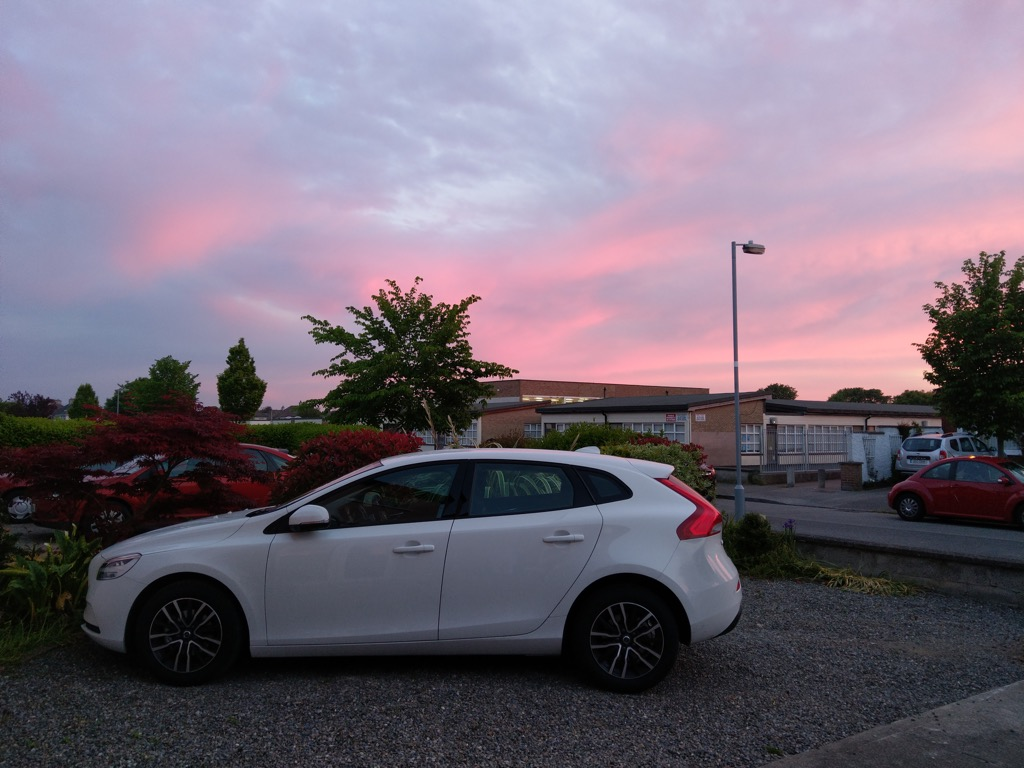
\includegraphics[width=\textwidth]{Sections/4InitialWork/4_images/run3_pic.jpg}
    \caption{} 
  \end{subfigure}
    \begin{subfigure}{0.1968\textwidth}
    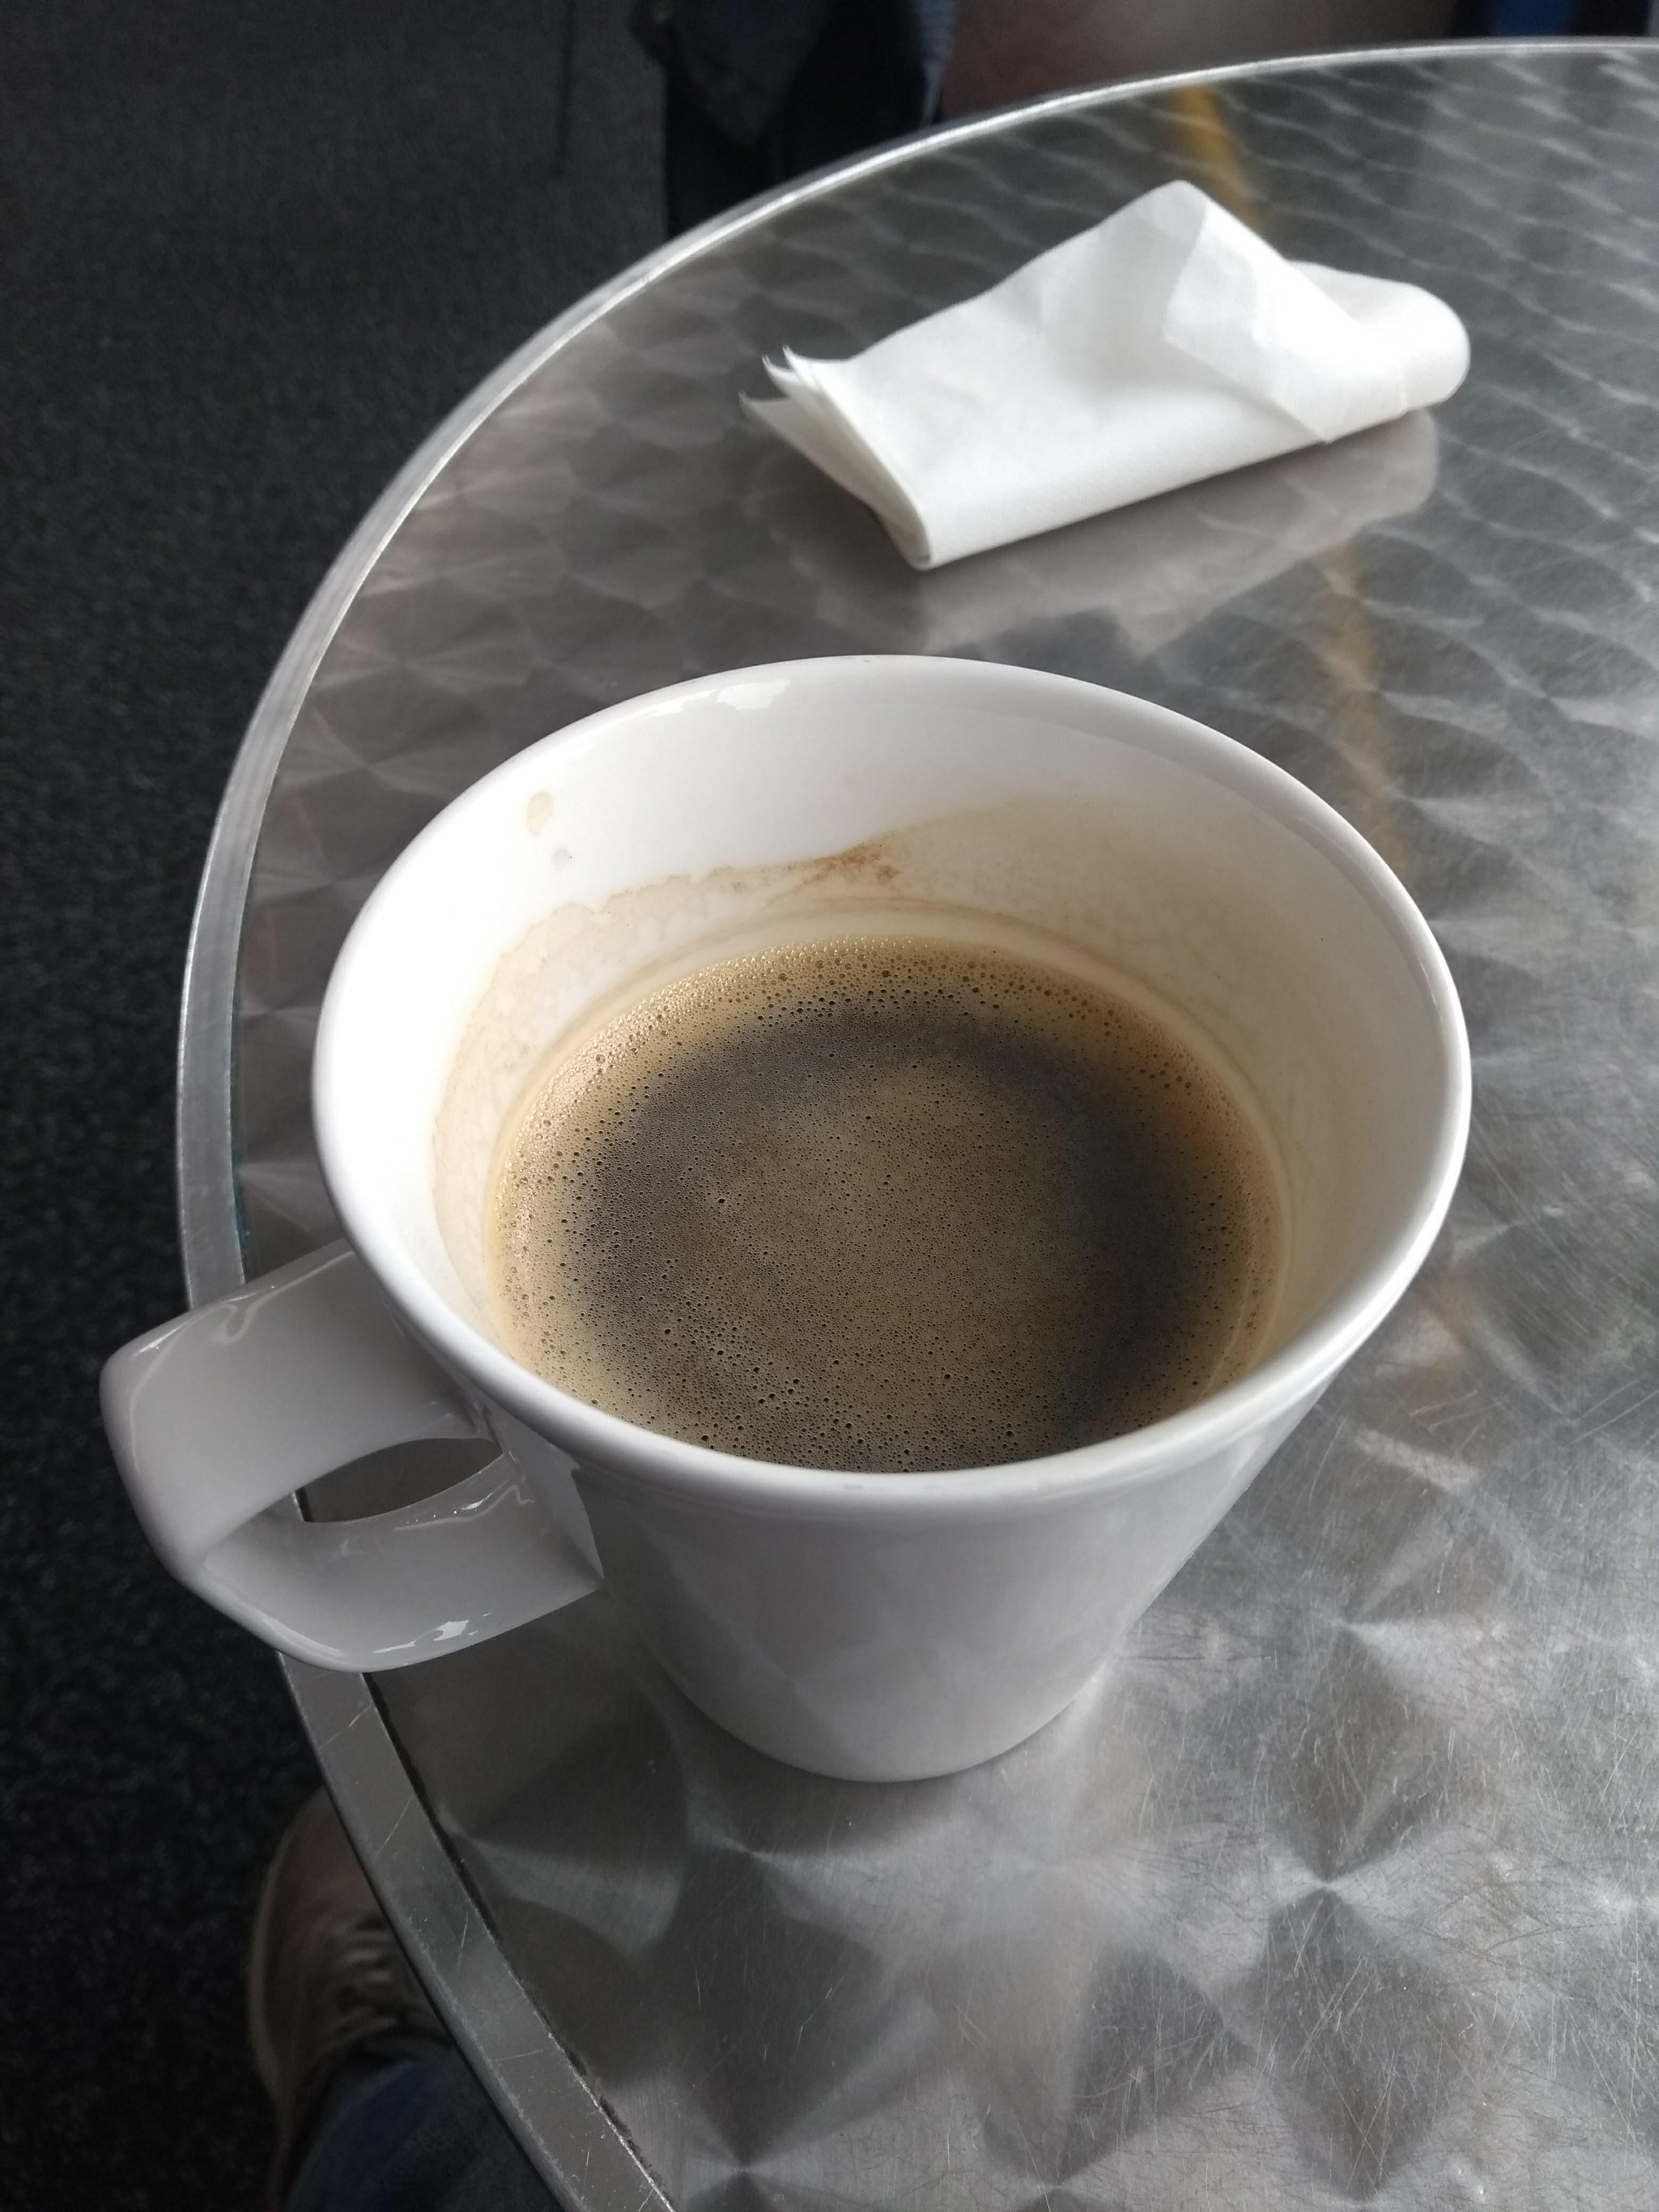
\includegraphics[width=\textwidth]{Sections/4InitialWork/4_images/run4_pic.jpg}
    \caption{}
   
  \end{subfigure}
  
    \caption{Samples of pictures used for image recognition preliminary experiences.}
    \label{fig:experi}
    \end{figure}


    \begin{itemize}
      \item \textbf{Obtained performance graphs in the image recognition tests}
    \end{itemize}
    
The following 3 images (Figure \ref{fig:exp1}, \ref{fig:exp2} and \ref{fig:exp3}) show three examples of the achieved performance of these algorithms in the processing of the pictures shown in Figure \ref{fig:experi}.

The graphs are structured in the following manner : the X axis represents the predictions, the Y axis represents the percentage probability certainty for the respective prediction and the color represents the algorithm evaluation and used.

The obtained results are discussed further down in this section.

\begin{figure}[H]
  \centering
  \captionsetup{justification=centering}
  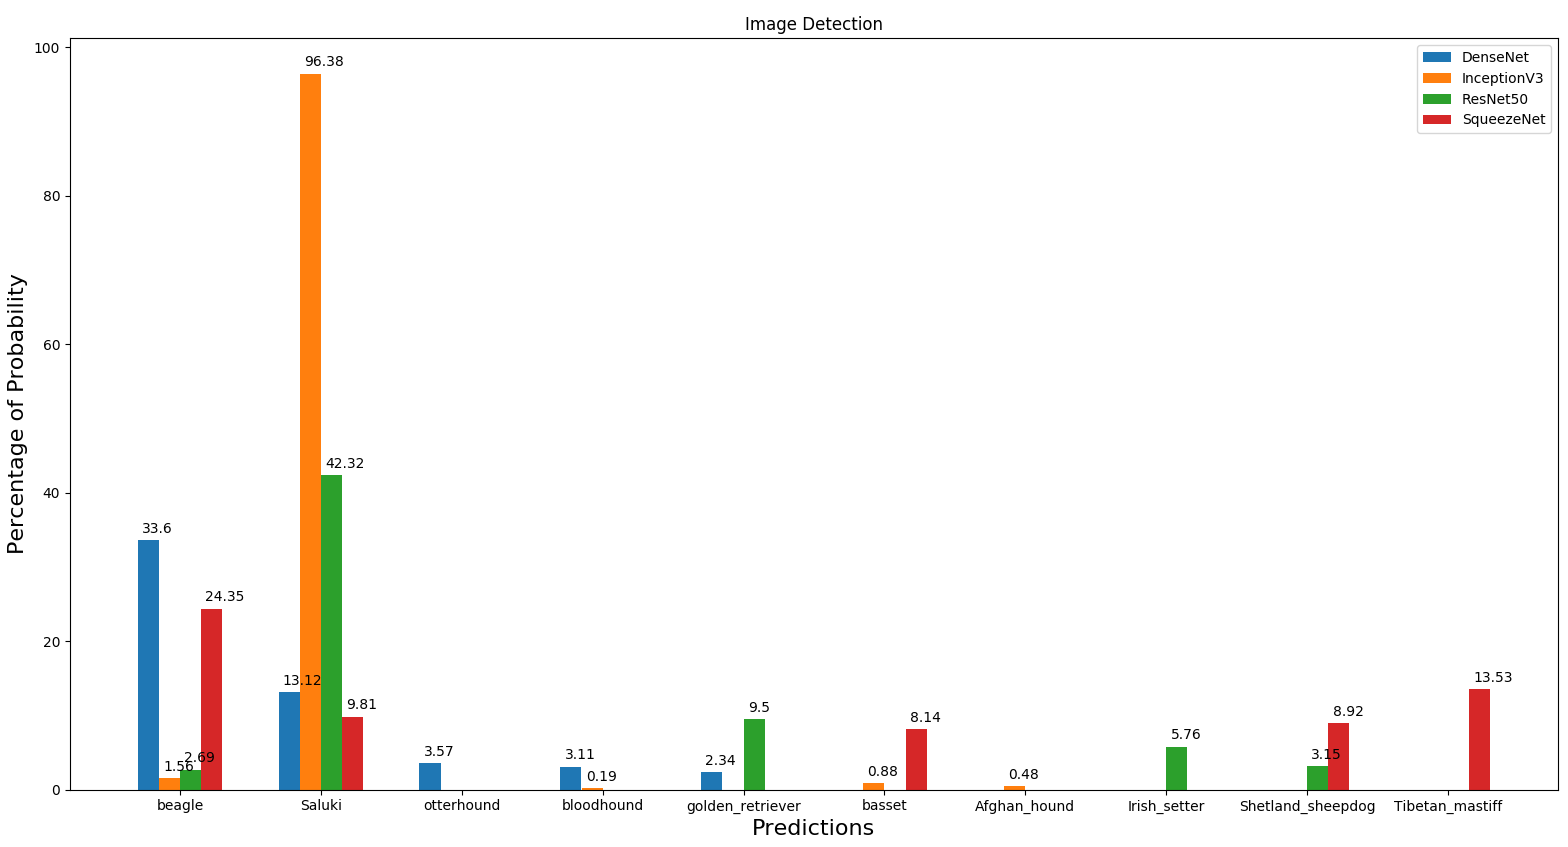
\includegraphics[width=\textwidth]{Sections/4InitialWork/4_images/run1_res.png}
  \caption{Achieved performance of different algorithms in the processing of Figure \ref{fig:experi} a).} 
  \label{fig:exp1}
\end{figure}



\begin{figure}[H]
  \centering
  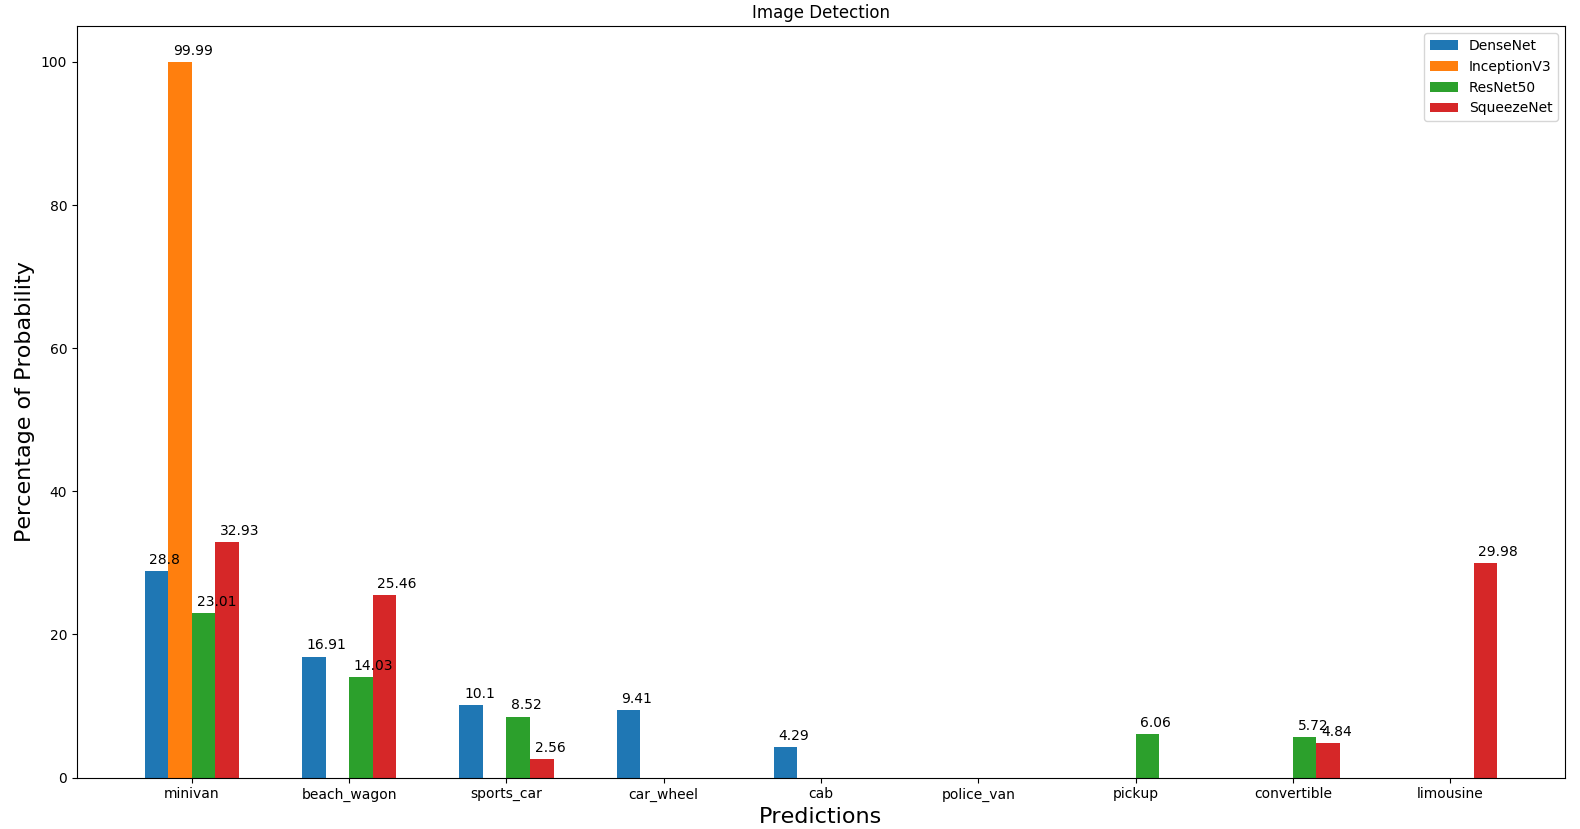
\includegraphics[width=\textwidth]{Sections/4InitialWork/4_images/run3_res.png}
  \caption{Achieved performance of different algorithms in the processing of Figure \ref{fig:experi} b).}
  \label{fig:exp2}
\end{figure}



\begin{figure}[H]
  \centering
  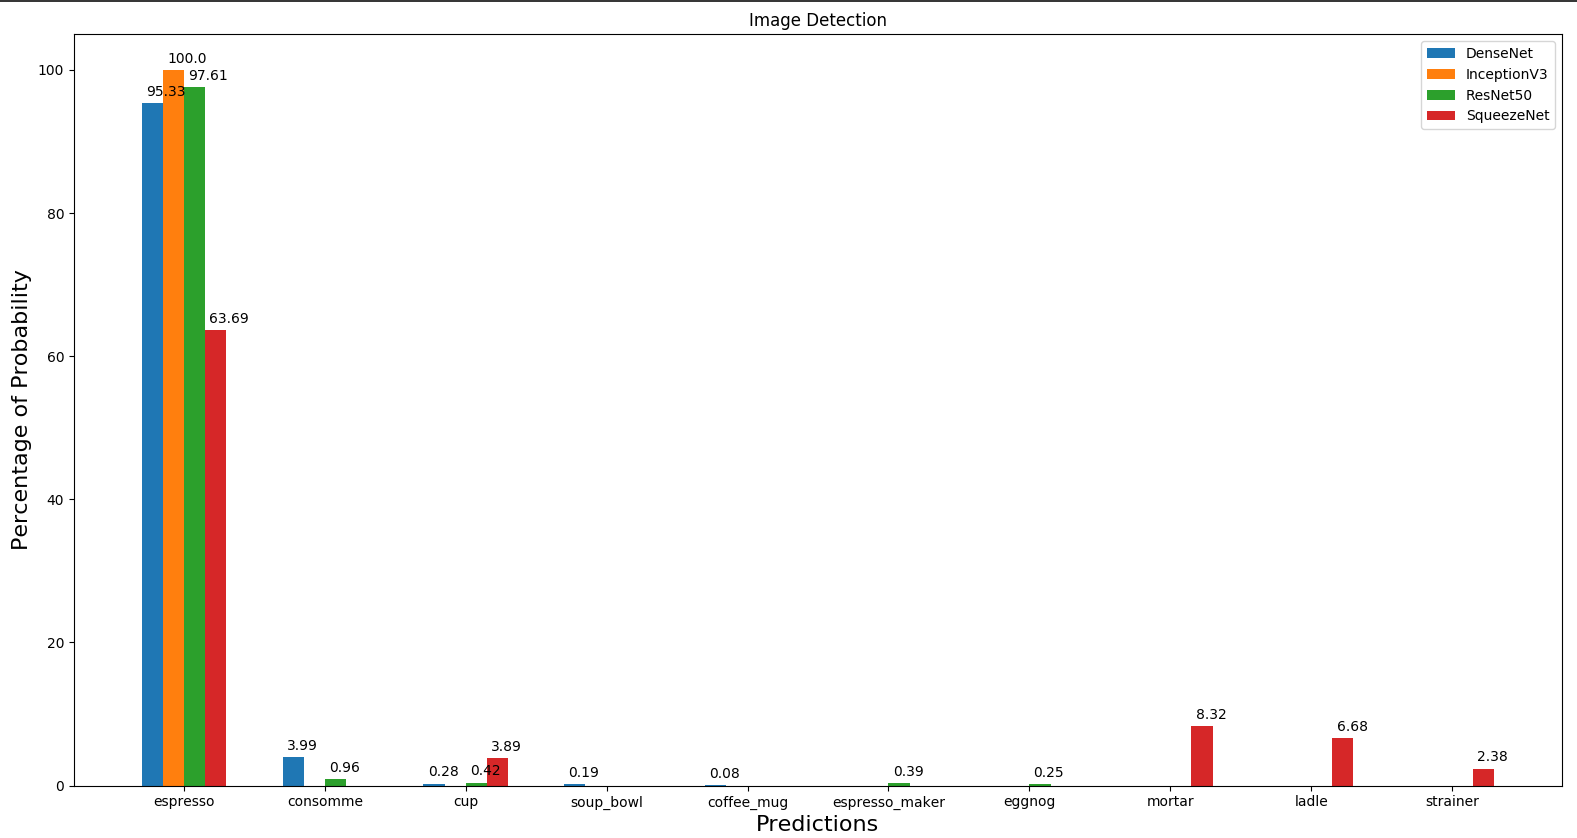
\includegraphics[width=\textwidth]{Sections/4InitialWork/4_images/run4_res.png}
  \caption{Achieved performance of different algorithms in the processing of Figure \ref{fig:experi} c).}
  \label{fig:exp3}
\end{figure}


\newpage


\begin{itemize}
  \item \textbf{Image recognition results analysis}
\end{itemize}





In the first example a picture of a dog (breed Saluki) is analysed. InceptionV3 is the best performer in the first run, predicting correctly with an efficiency of 96.38\% and out performing the other 3 neural networks by a large margin, being that the second best is the ResNet50 with an efficiency of 42.32\%.

For the second example a picture of a car was processed. InceptionV3 predicted with a 99.99\% that the car was a minivan. The shown car is not a minivan but its similar to one, so it is possible to assume that the prediction is correct.

The final example a picture of an espresso coffee is analysed. In this example all image recognition algorithms predicted correctly that the image represents an espresso. However, SquezeeNet only achieved 63.88\% efficiency while InceptionV3 predicted with 100.0\% efficiency.

From the 3 examples that were shown, it is clear that the inceptionV3 algorithm achieved the best results and out performed the other algorithms.






  %%%%%%%%%%%%%%%%%%%%%%%%%%%%%%%%%%%%% OBJECT RECOGNITION   %%%%%%%%%%%%%%%%%%%%%%%%%%%%%%%%%%%%%

  \subsection{Object Detection Preliminary Experiences}
  \label{sec:object_test}

  ImageAI provides 3 different models trained on the COCO dataset for object detection that are able to identify up to 80 of the most common objects in everyday life. Figure \ref{fig:labels} illustrates all of the objects that these models are able to detect in an image. The models that are provided include RetinaNet, YOLOv3 and TinyYOLOv3. \cite{ImageAI}.
  

  

    \begin{figure}[htb]
      \centering
      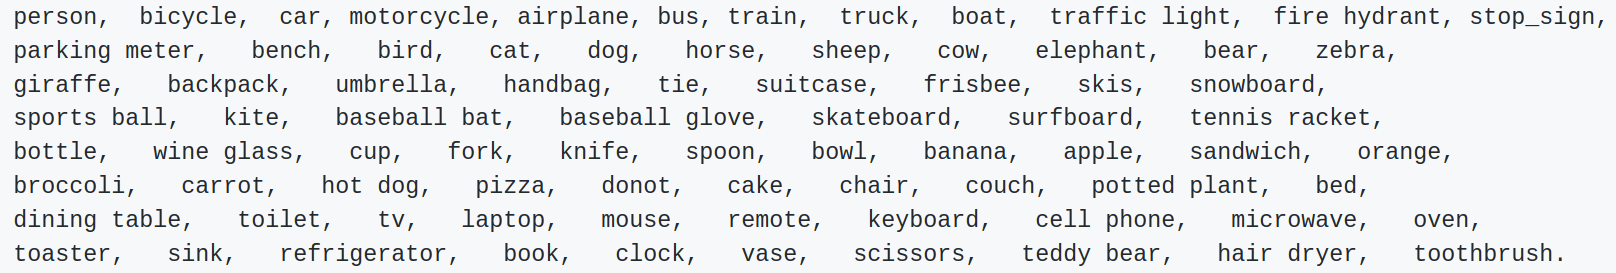
\includegraphics[width = \textwidth]{Sections/4InitialWork/4_images_random/detections.png}
      \caption{Available labels for detection. }
      \label{fig:labels} 
  \end{figure}

  The next pages present the tests done which are structured in the following way: on the left is the picture with the respective detections and on the right is an image with a graph representation of the detections. The color represents the detected object (label) which is the same in both images. The analysis of the achieved results are discussed later in Section \ref{ch:wordclouds}.

  The pictures used for the testing of the described models were the following:

\begin{figure}[H]
  \centering
  \captionsetup{justification=centering}

  \begin{subfigure}{0.3\textwidth}
  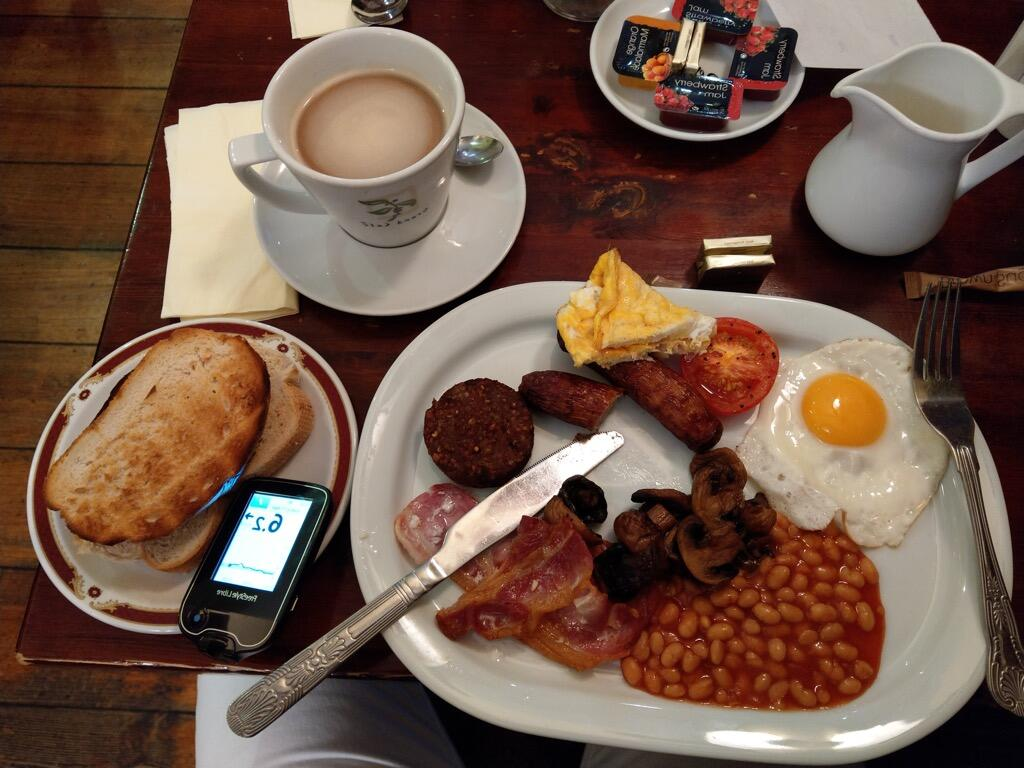
\includegraphics[width=\textwidth]{Sections/4InitialWork/4_images_obj_run1/photo.jpg} 
  \end{subfigure}
  \begin{subfigure}{0.3\textwidth}
  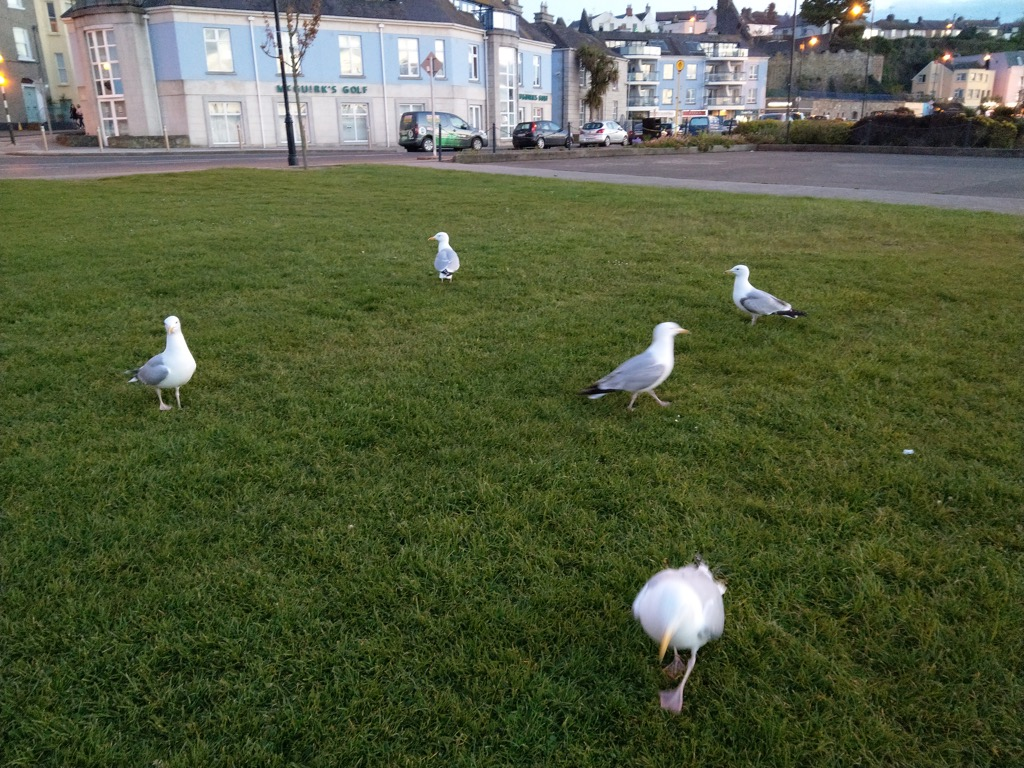
\includegraphics[width=\textwidth]{Sections/4InitialWork/4_images_obj_run3/photo.jpg}
  \end{subfigure}
  \begin{subfigure}{0.3\textwidth}
  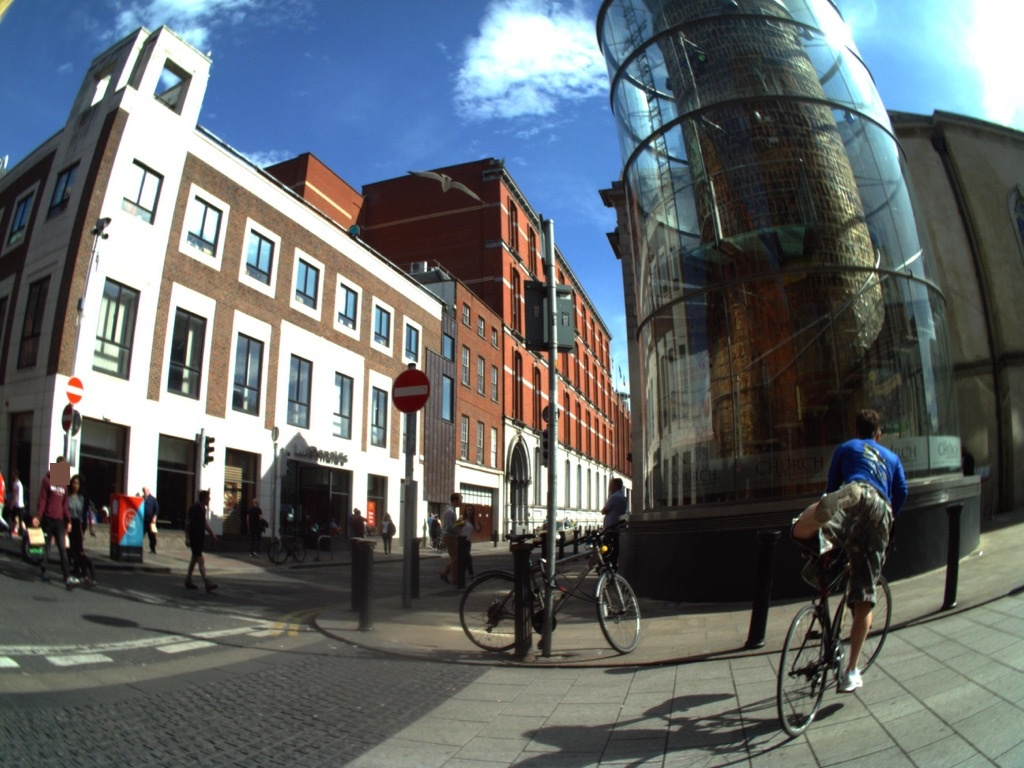
\includegraphics[width=\textwidth]{Sections/4InitialWork/4_images_obj_run4/photo.jpg}
  \end{subfigure}

  \caption{ 
  Sample pictures used for testing the object recognition models.}
  \end{figure}



  evaluation and
    
  \begin{itemize}
    \item \textbf{Detection Experience Number 1}
  \end{itemize}

    

      \begin{figure}[H]
        \centering
        \captionsetup{justification=centering}

        \begin{subfigure}{0.29\textwidth}
        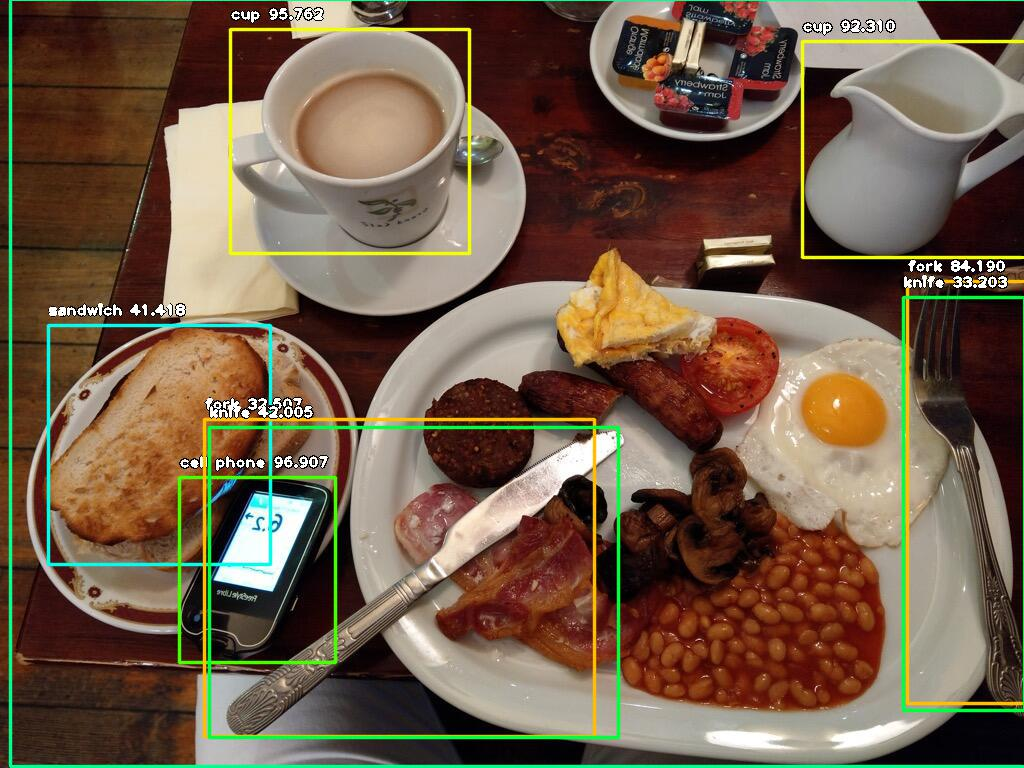
\includegraphics[width=\textwidth]{Sections/4InitialWork/4_images_obj_run1/retinaNet.jpg} 
        \caption{}
        \end{subfigure}
        \begin{subfigure}{0.65\textwidth}
        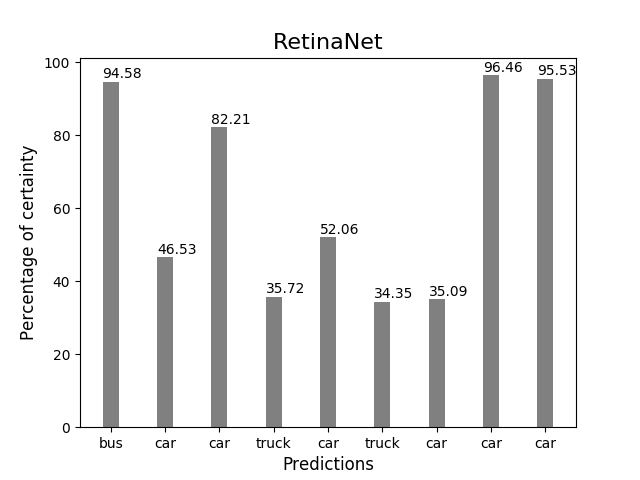
\includegraphics[width=\textwidth]{Sections/4InitialWork/4_images_obj_run1/retinaNet_graph.png}
        \caption{}
        \end{subfigure}
        
        \caption{ 
        Test run 1 with RetinaNet; a) Analysed picture with detections; b) Achieved performance on detections. }
        \end{figure}
    

      
        \begin{figure}[H]
          \centering
          \captionsetup{justification=centering}
  
          \begin{subfigure}{0.29\textwidth}
          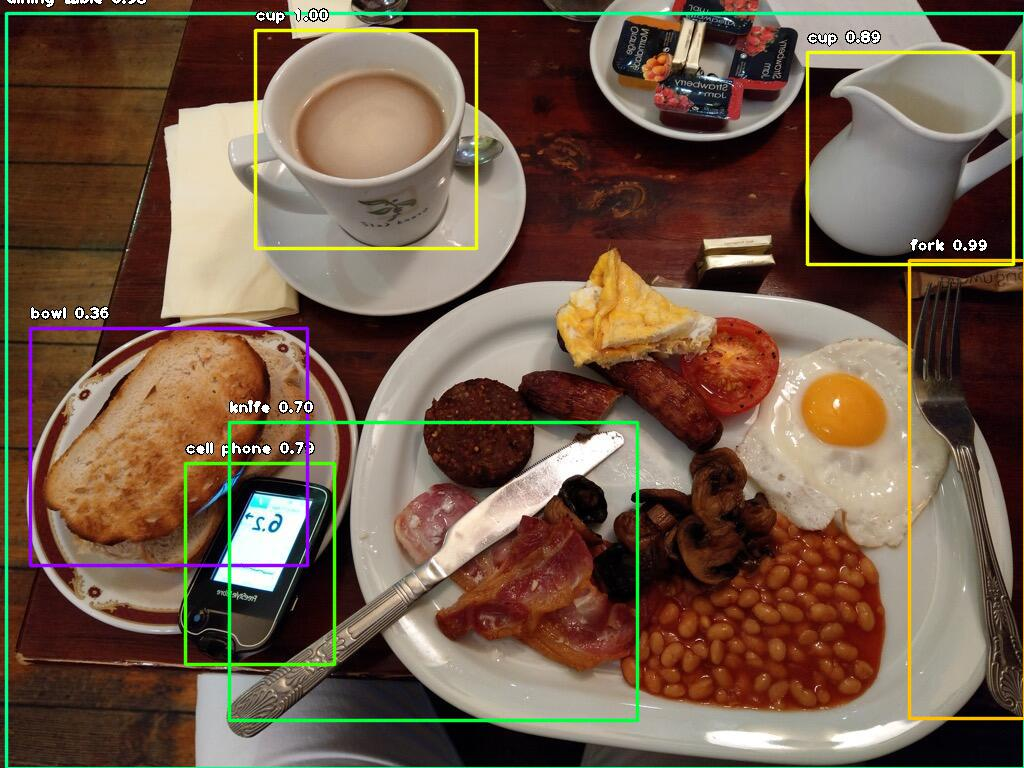
\includegraphics[width=\textwidth]{Sections/4InitialWork/4_images_obj_run1/yolo.jpg} 
          \caption{}
          \end{subfigure}
          \begin{subfigure}{0.65\textwidth}
          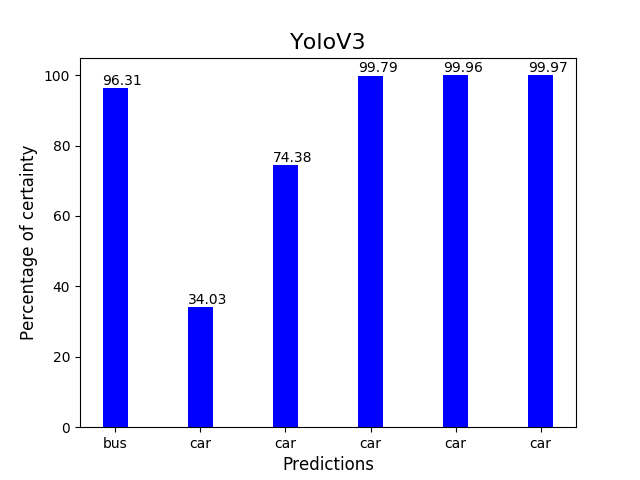
\includegraphics[width=\textwidth]{Sections/4InitialWork/4_images_obj_run1/yolo_graph.png}
          \caption{}
          \end{subfigure}
          
          \caption{ 
          Test run 1 with YOLOv3; a) Analysed picture with detections; b) Achieved performance on detections. }
          \end{figure}
      


          \begin{figure}[H]
            \centering
            \captionsetup{justification=centering}
    
            \begin{subfigure}{0.29\textwidth}
            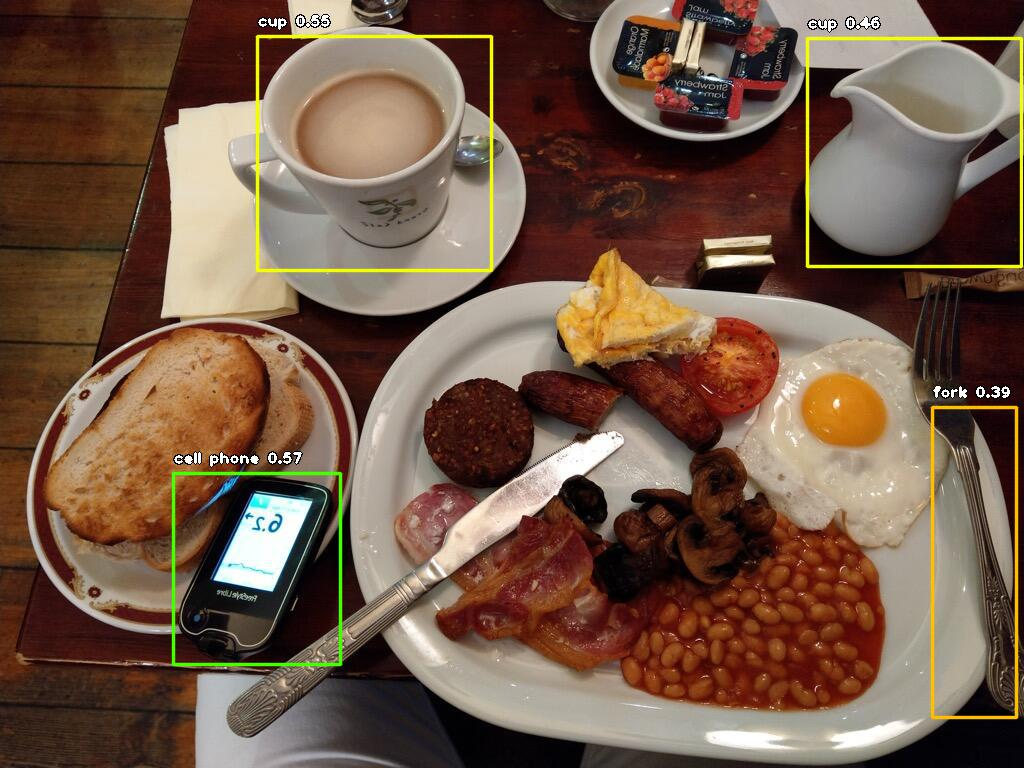
\includegraphics[width=\textwidth]{Sections/4InitialWork/4_images_obj_run1/yolo_tiny.jpg} 
            \caption{}
            \end{subfigure}
            \begin{subfigure}{0.4\textwidth}
            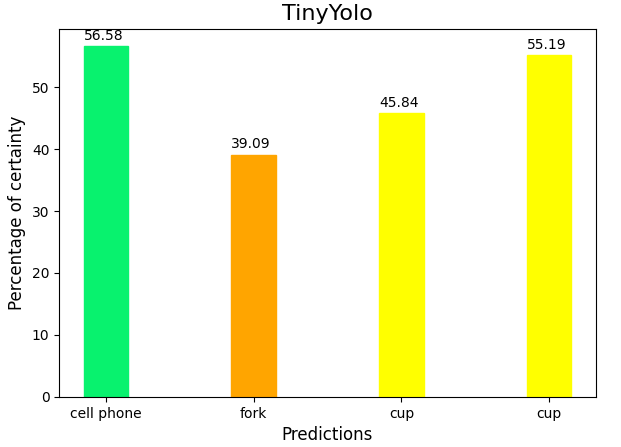
\includegraphics[width=\textwidth]{Sections/4InitialWork/4_images_obj_run1/tiny_yolo_graph.png}
            \caption{}
            \end{subfigure}
            
            \caption{ 
            Test run 1 with TinyYolo; a) Analysed picture with detections; b) Achieved performance on detections. }
            \end{figure}

      \newpage

  %%%%%%%%%%%%%%%%%%%%%%%%%%%%%%%%%%%%% run2   %%%%%%%%%%%%%%%%%%%%%%%%%%%%%%%%%%%%%
      
  \begin{itemize}
    \item \textbf{Detection Experience Number 2}
  \end{itemize}

    

      \begin{figure}[H]
        \centering
        \captionsetup{justification=centering}

        \begin{subfigure}{0.29\textwidth}
        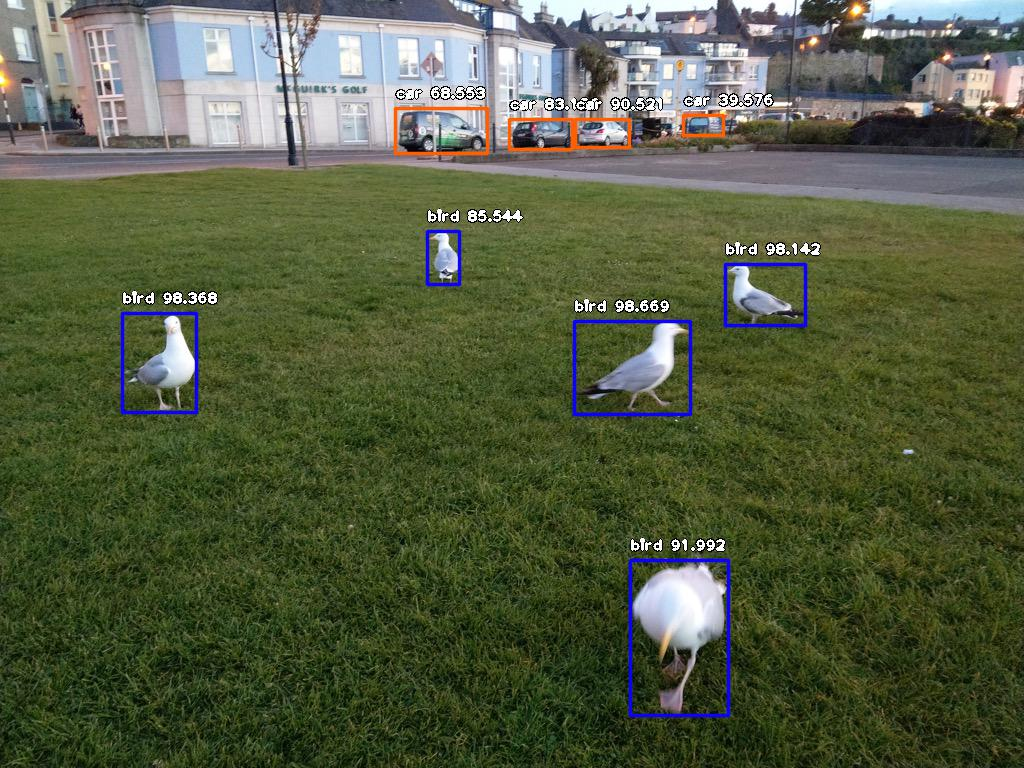
\includegraphics[width=\textwidth]{Sections/4InitialWork/4_images_obj_run3/retinaNet.jpg} 
        \caption{}
        \end{subfigure}
        \begin{subfigure}{0.65\textwidth}
        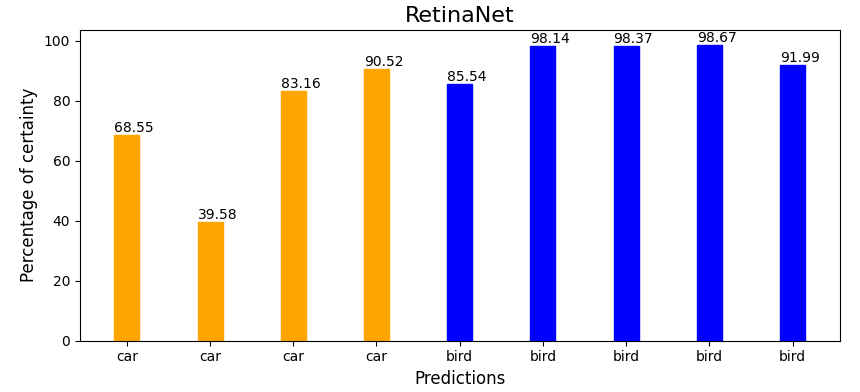
\includegraphics[width=\textwidth]{Sections/4InitialWork/4_images_obj_run3/retinaNet_graph.png}
        \caption{}
        \end{subfigure}
        
        \caption{ 
        Test run 2 with RetinaNet; a) Analysed picture with detections; b) Achieved performance detections. }
        \end{figure}



        \begin{figure}[H]
          \centering
          \captionsetup{justification=centering}
  
          \begin{subfigure}{0.29\textwidth}
          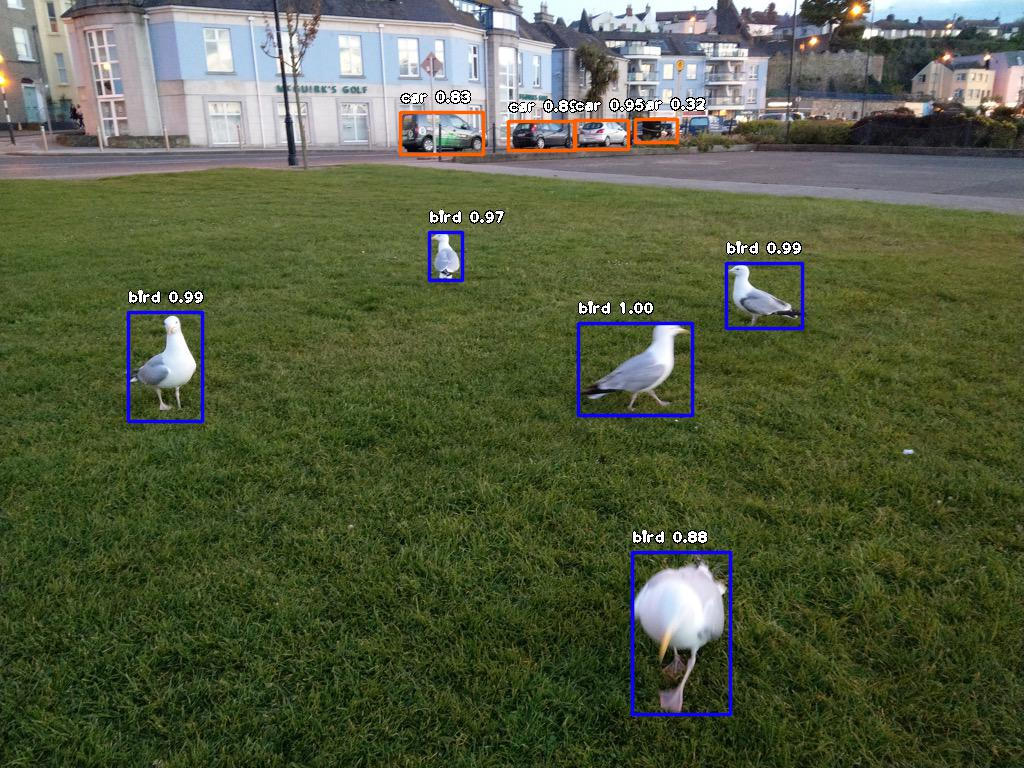
\includegraphics[width=\textwidth]{Sections/4InitialWork/4_images_obj_run3/yolo.jpg} 
          \caption{}
          \end{subfigure}
          \begin{subfigure}{0.65\textwidth}
          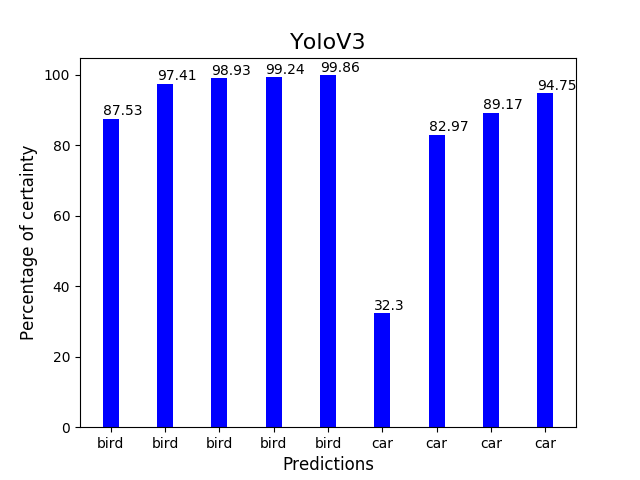
\includegraphics[width=\textwidth]{Sections/4InitialWork/4_images_obj_run3/yolo_graph.png}
          \caption{}
          \end{subfigure}
          
          \caption{ 
          Test run 2 with YoloV3 model; a) Analysed picture with detections; b) Achieved performance on detections. }
          \end{figure}
  

          \begin{figure}[H]
            \centering
            \captionsetup{justification=centering}
    
            \begin{subfigure}{0.29\textwidth}
            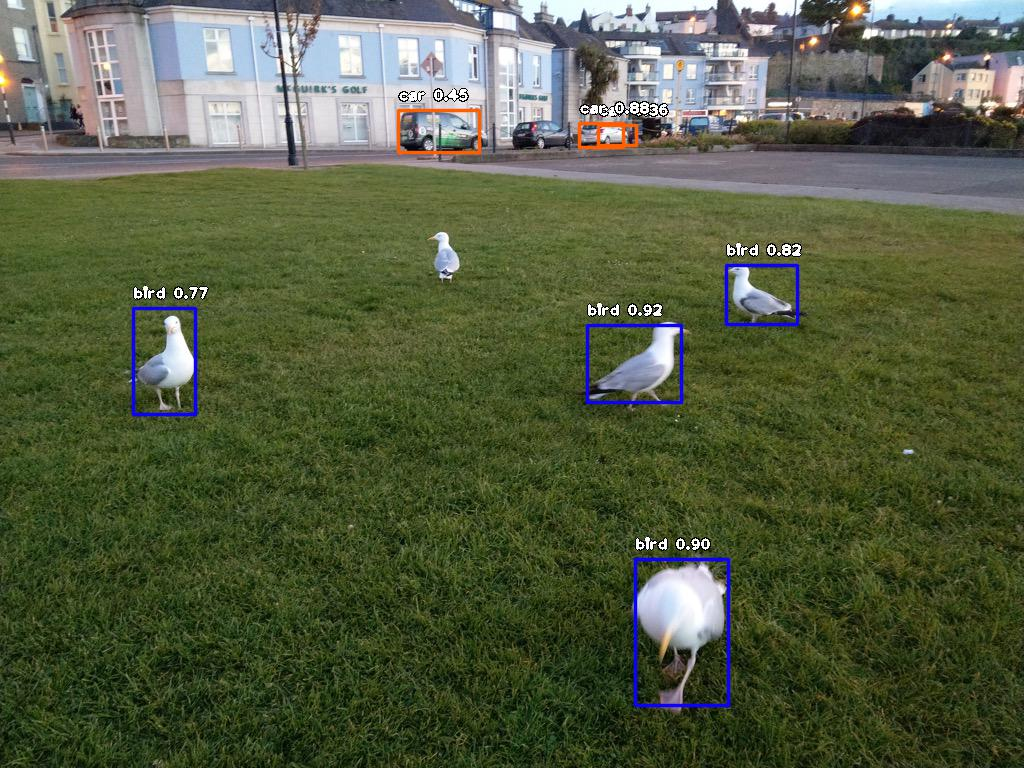
\includegraphics[width=\textwidth]{Sections/4InitialWork/4_images_obj_run3/yolo_tiny.jpg} 
            \caption{}
            \end{subfigure}
            \begin{subfigure}{0.6\textwidth}
            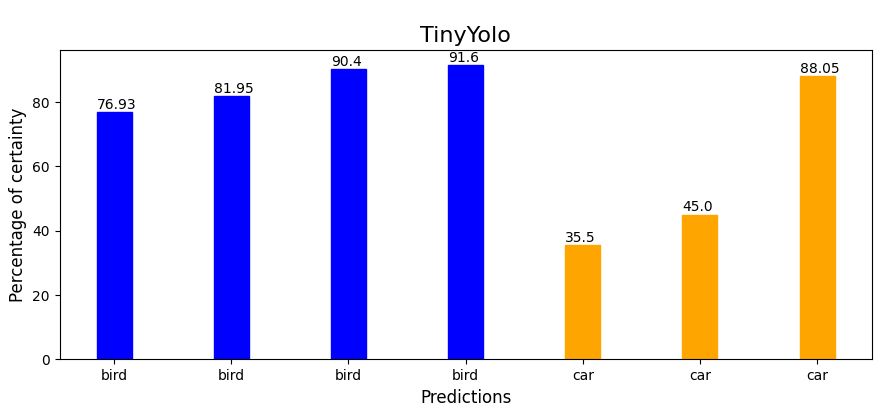
\includegraphics[width=\textwidth]{Sections/4InitialWork/4_images_obj_run3/yolo_tiny_graph.png}
            \caption{}
            \end{subfigure}
            
            \caption{ 
            Test run 2 with TinyYolo; a) Analysed picture with detections; b) Achieved performance on detections. }
            \end{figure}

      \newpage

      \begin{itemize}
        \item \textbf{Detection Experience Number 3}
      \end{itemize}
    

      \begin{figure}[H]
        \centering
        \captionsetup{justification=centering}

        \begin{subfigure}{0.29\textwidth}
        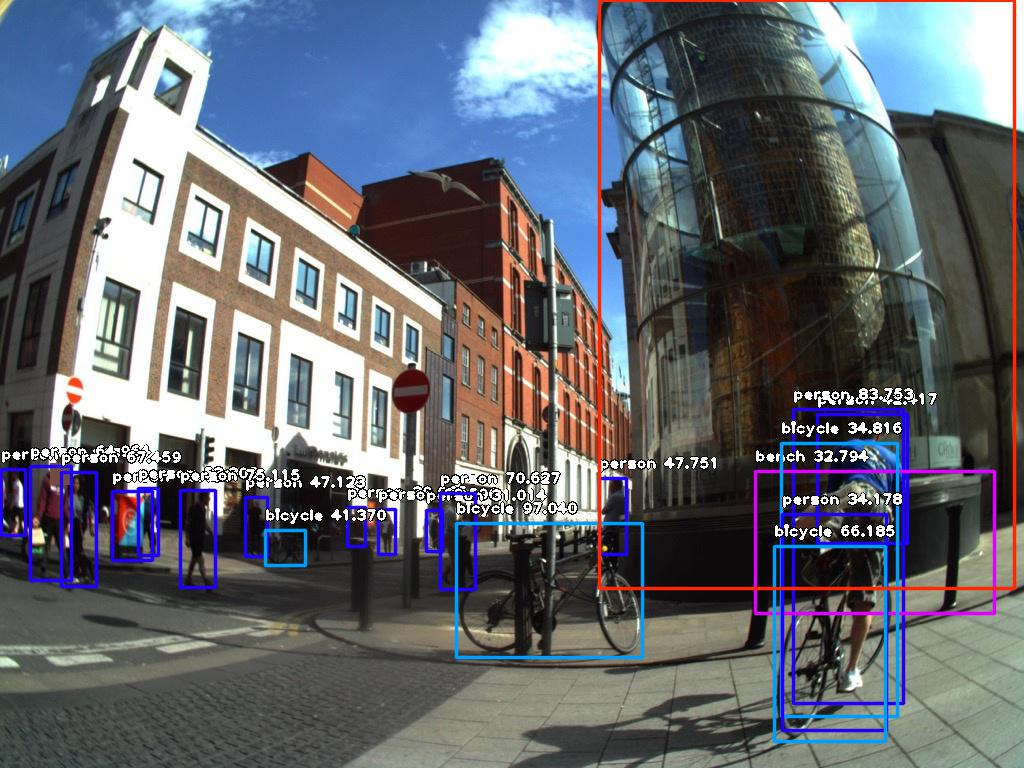
\includegraphics[width=\textwidth]{Sections/4InitialWork/4_images_obj_run4/retinaNet.jpg} 
        \caption{}
        \end{subfigure}
        \begin{subfigure}{0.7\textwidth}
        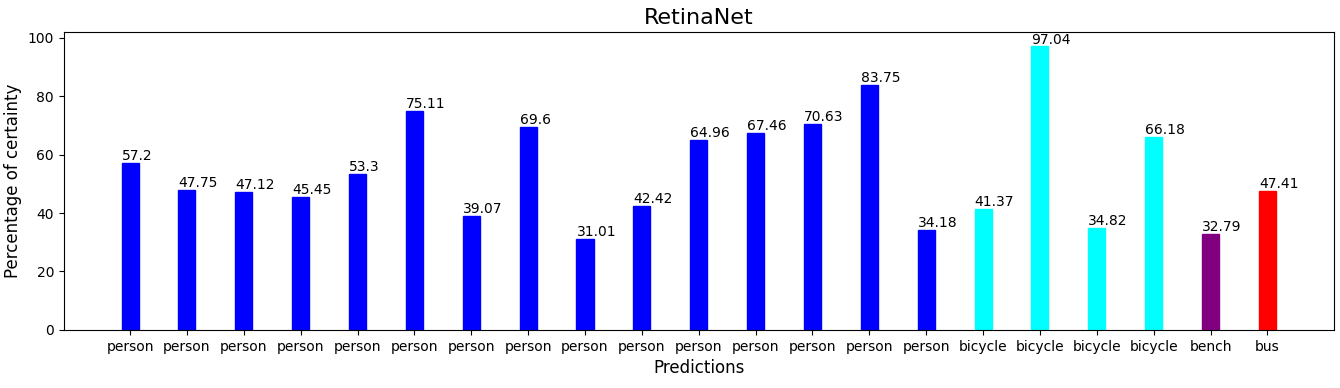
\includegraphics[width=\textwidth]{Sections/4InitialWork/4_images_obj_run4/retinaNet_graph.png}
        \caption{}
        \end{subfigure}
        
        \caption{ 
        Test run 3 with RetinaNet; a) Analysed picture with detections; b) Achieved performance detections. }
        \end{figure}



        \begin{figure}[H]
          \centering
          \captionsetup{justification=centering}
  
          \begin{subfigure}{0.29\textwidth}
          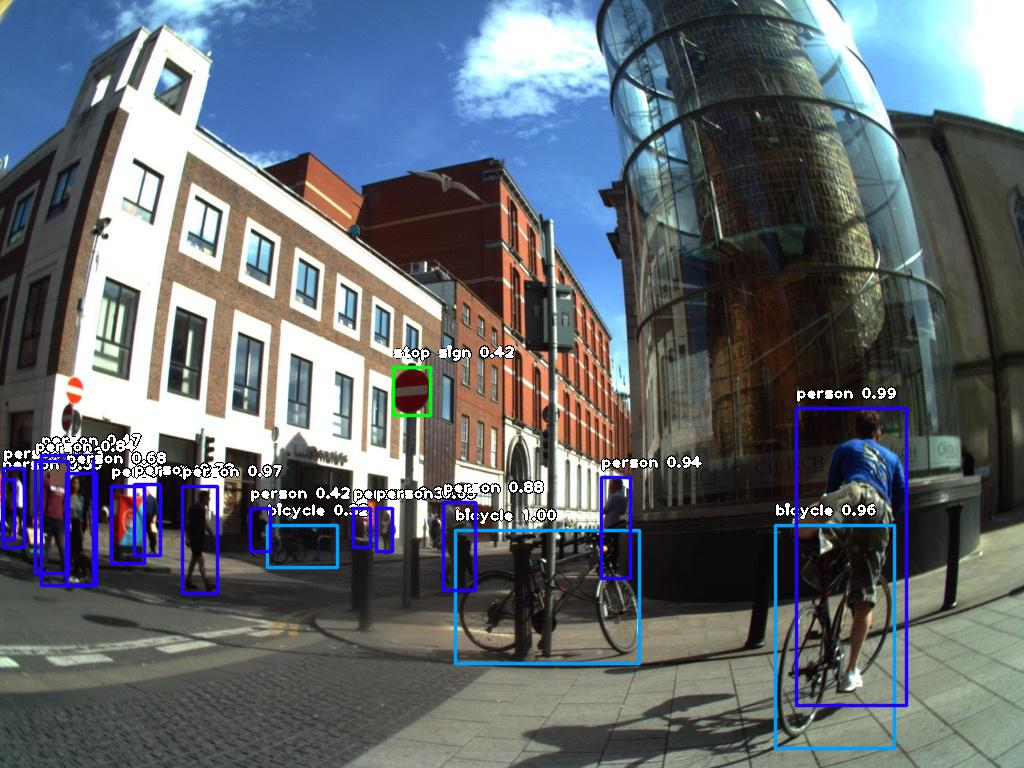
\includegraphics[width=\textwidth]{Sections/4InitialWork/4_images_obj_run4/yolo.jpg} 
          \caption{}
          \end{subfigure}
          \begin{subfigure}{0.7\textwidth}
          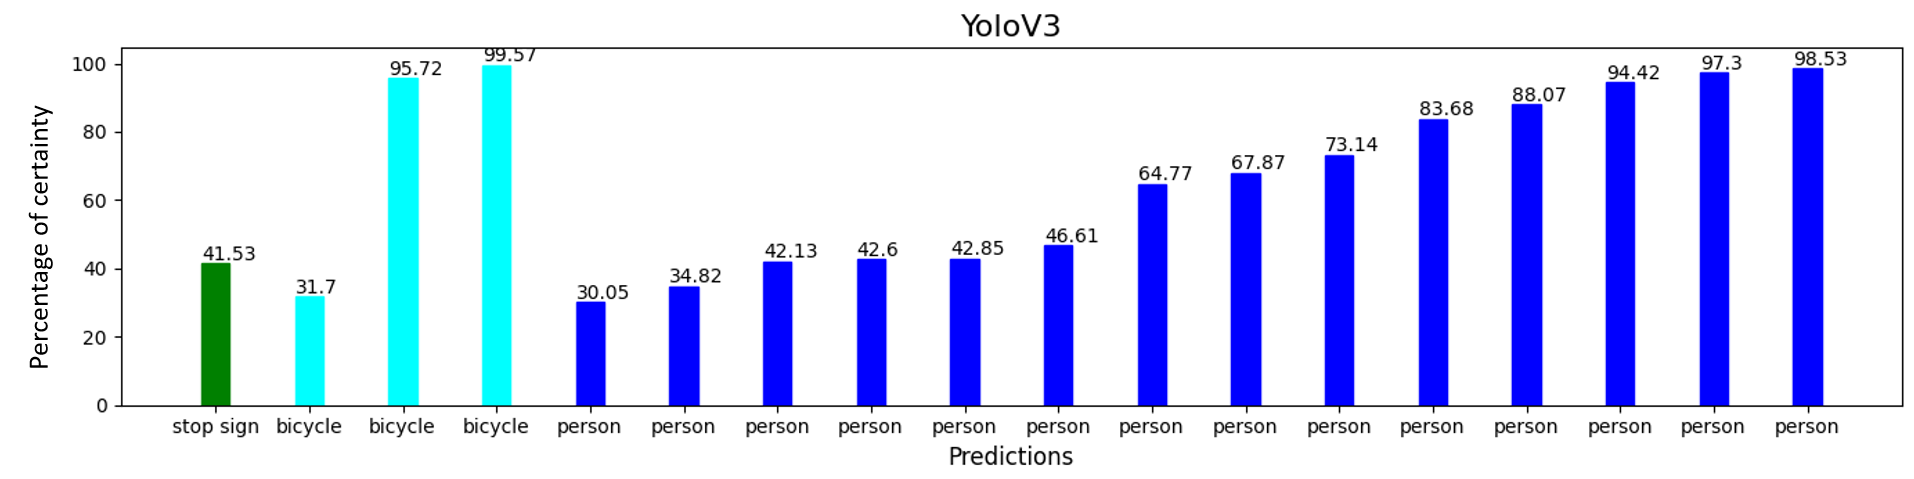
\includegraphics[width=\textwidth]{Sections/4InitialWork/4_images_obj_run4/yolo_graph.png}
          \caption{}
          \end{subfigure}
          
          \caption{ 
          Test run 3 with YoloV3 model; a) Analysed picture with detections; b) Achieved performance on detections. }
          \end{figure}
  

          \begin{figure}[H]
            \centering
            \captionsetup{justification=centering}
    
            \begin{subfigure}{0.29\textwidth}
            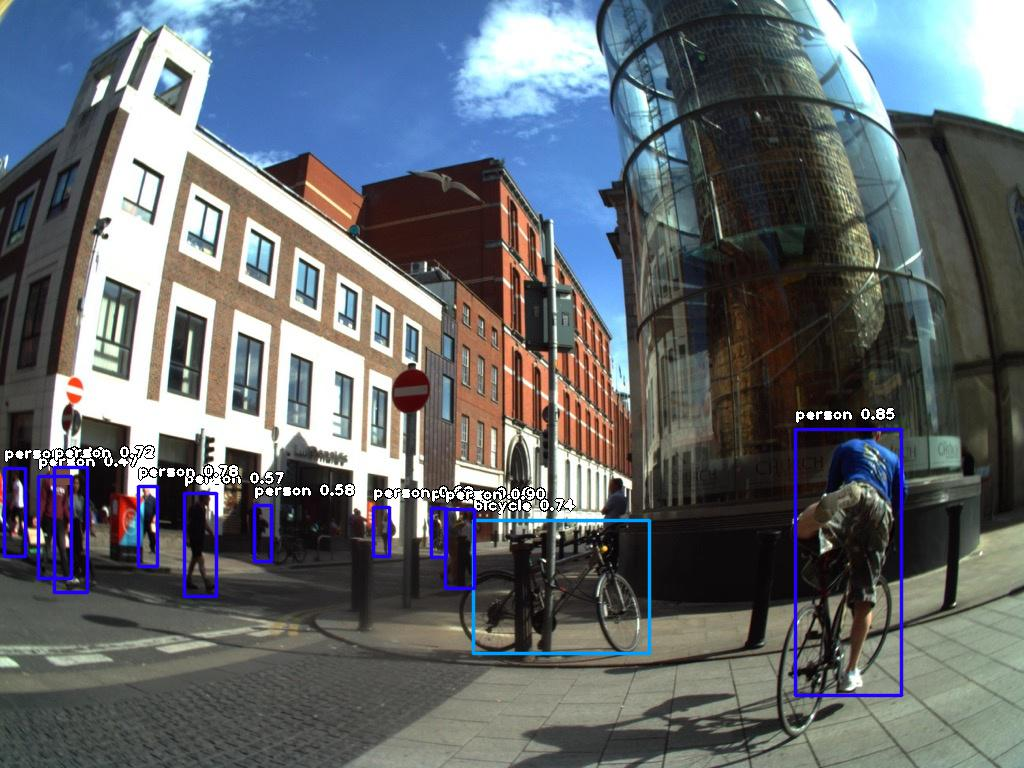
\includegraphics[width=\textwidth]{Sections/4InitialWork/4_images_obj_run4/yolo_tiny.jpg} 
            \caption{}
            \end{subfigure}
            \begin{subfigure}{0.65\textwidth}
            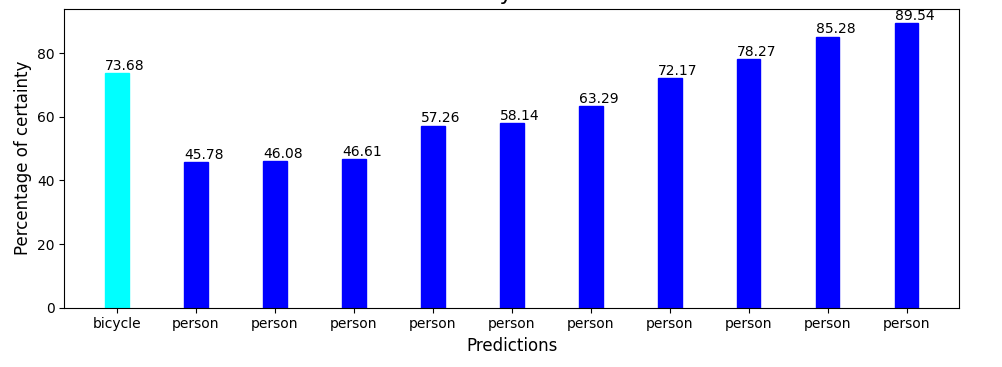
\includegraphics[width=\textwidth]{Sections/4InitialWork/4_images_obj_run4/tiny_yolo_graph.png}
            \caption{}
            \end{subfigure}
            
            \caption{ 
            Test run 3 with TinyYolo; a) Analysed picture with detections; b) Achieved performance on detections. }
            \end{figure}


    \newpage

    \subsection{Object Detection Word Clouds Generation Test Run}
    \label{ch:wordclouds}
    In order to make the labels extraction more easily visible and still achieve some degree of performance comparison between the 3 object detection models word clouds were generated. In a word cloud, the bigger a word is the more times that label was detected in the pictures. For this test 6 previously chosen images with identical setting were processed in order to generate 1 word cloud with all the extracted labels.

    The following images were used for word cloud generation:
    
   


    \begin{figure}[H]
      \begin{subfigure}{\linewidth}
      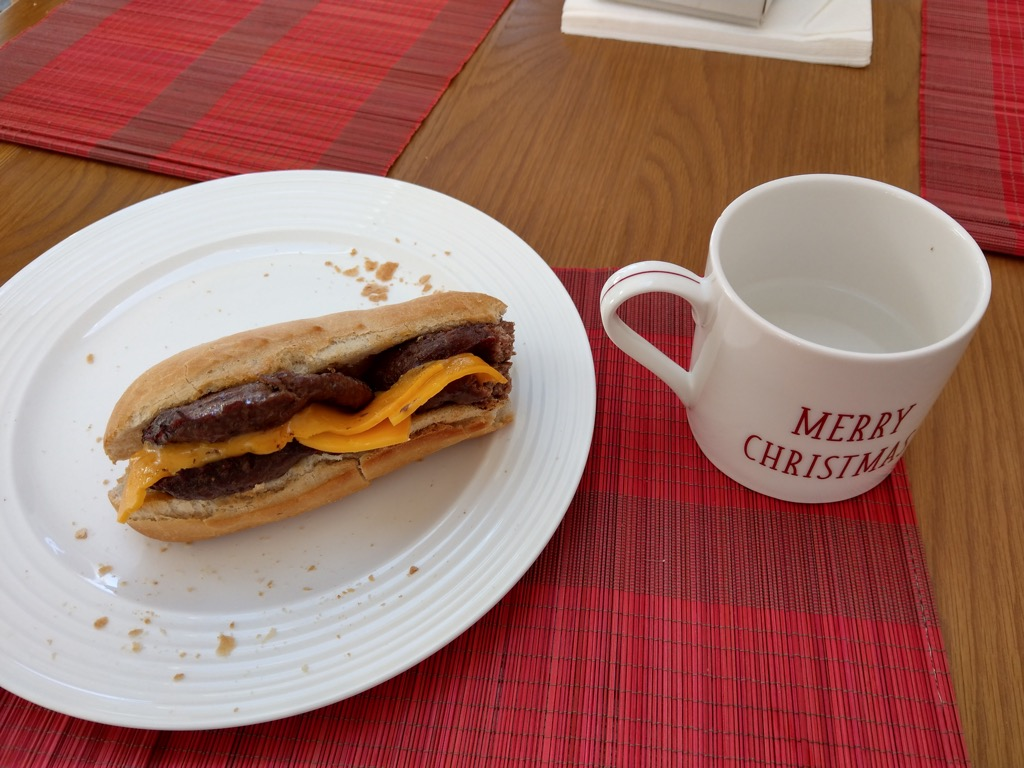
\includegraphics[width=.3\linewidth]{Sections/4InitialWork/4_images_wordcloud/photo1.jpg}\hfill
      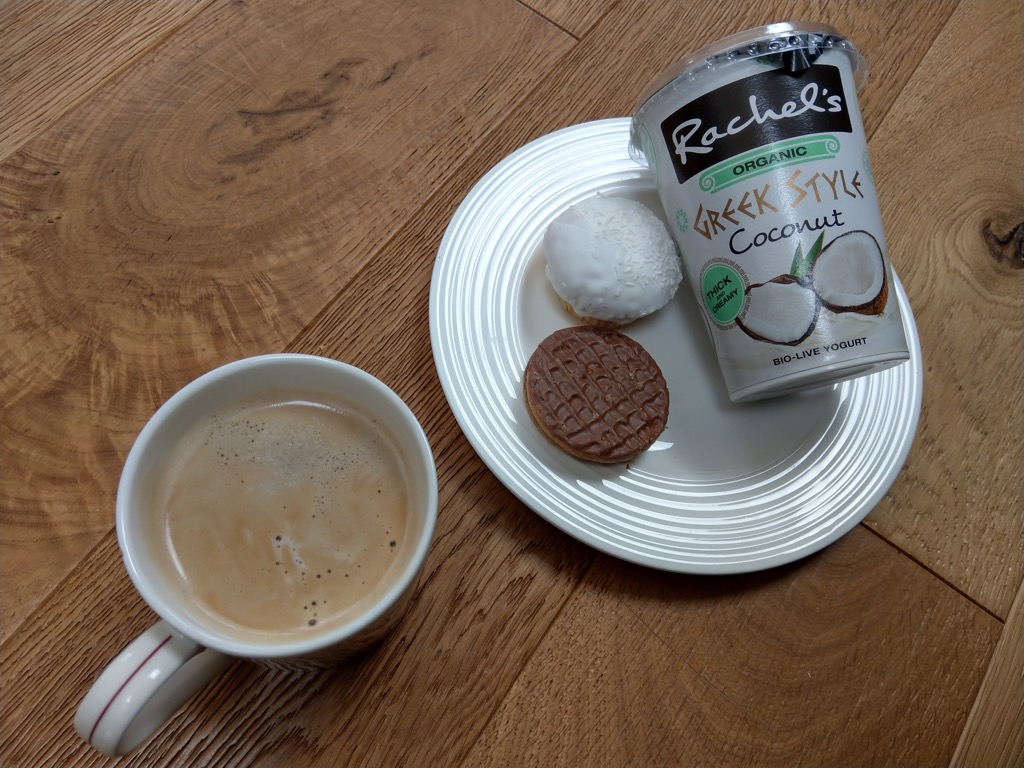
\includegraphics[width=.3\linewidth]{Sections/4InitialWork/4_images_wordcloud/photo2.jpg}\hfill
      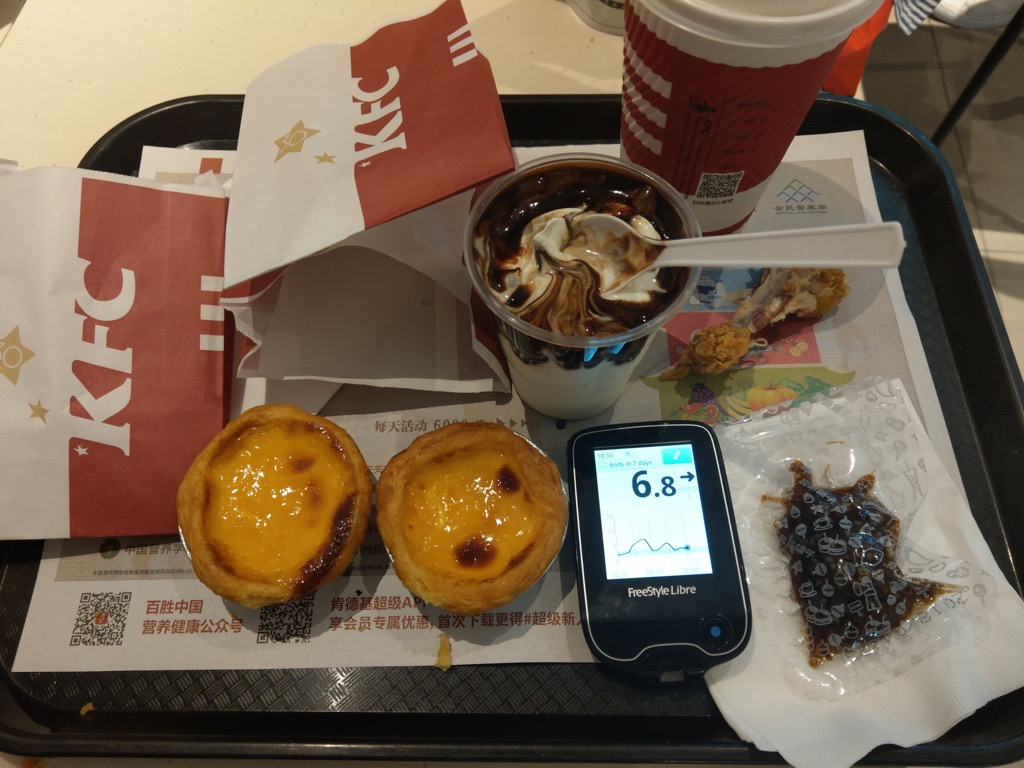
\includegraphics[width=.3\linewidth]{Sections/4InitialWork/4_images_wordcloud/photo7.jpg}
      \end{subfigure}\par\medskip
      \begin{subfigure}{\linewidth}
      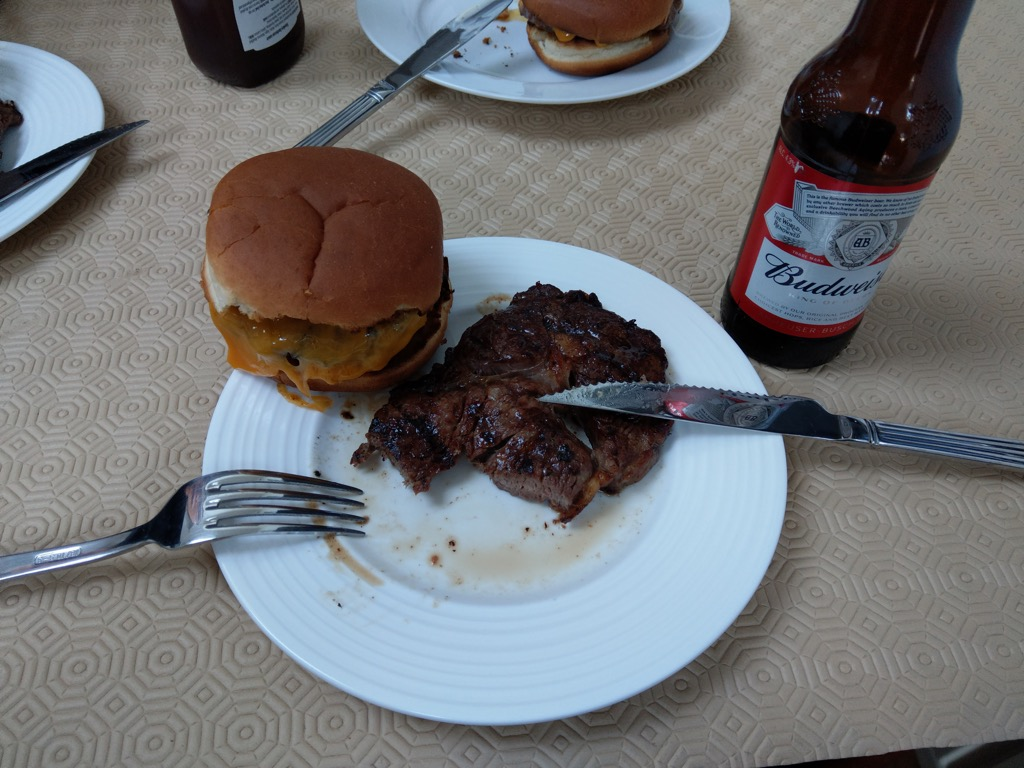
\includegraphics[width=.3\linewidth]{Sections/4InitialWork/4_images_wordcloud/photo4.jpg}\hfill
      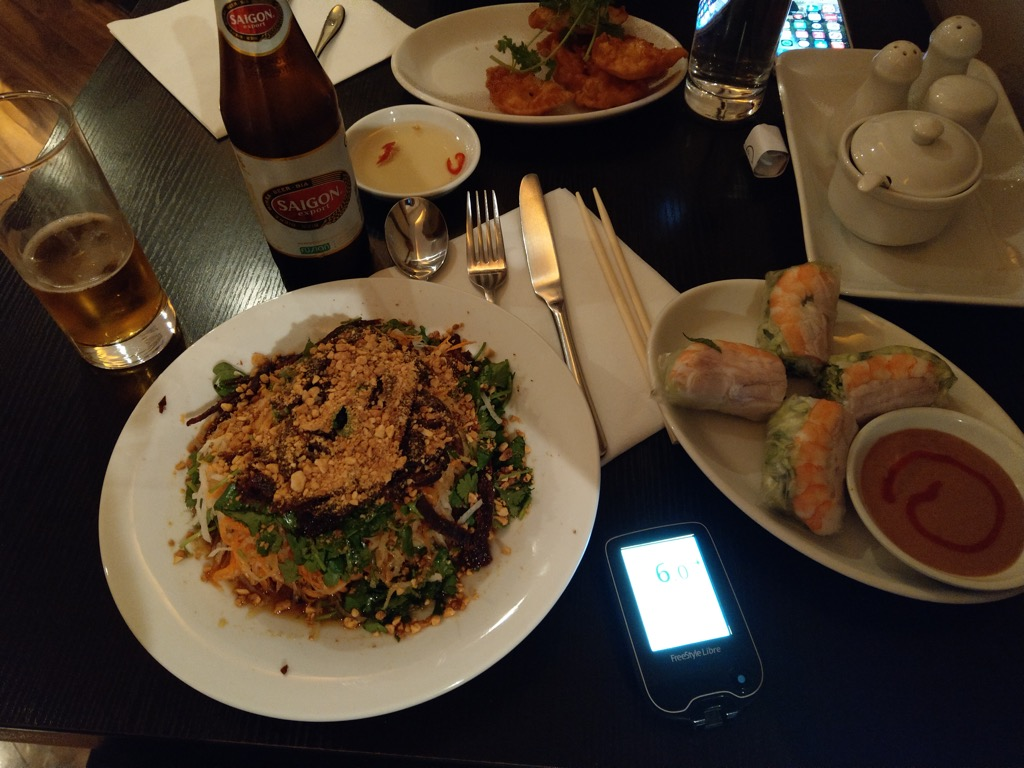
\includegraphics[width=.3\linewidth]{Sections/4InitialWork/4_images_wordcloud/photo5.jpg}\hfill
      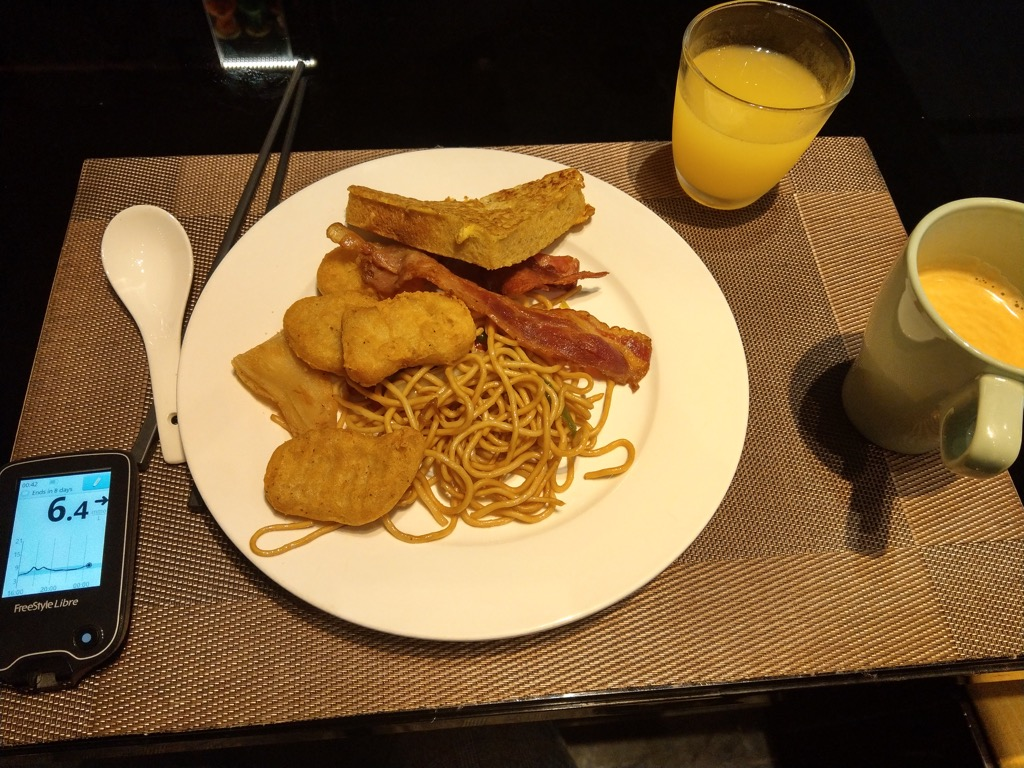
\includegraphics[width=.3\linewidth]{Sections/4InitialWork/4_images_wordcloud/photo6.jpg}
      \end{subfigure}\par\medskip
      \caption{Used images for word cloud generation.}
    \end{figure}


    \begin{itemize}
      \item \textbf{Generated Word Clouds}
    \end{itemize}
    


    \begin{figure}[H]
      \centering
      \captionsetup{justification=centering}
    
      \begin{subfigure}{0.33\textwidth}
      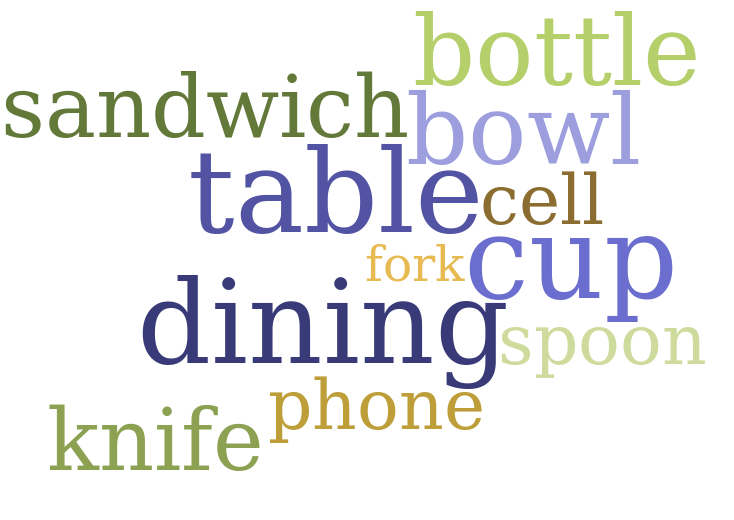
\includegraphics[width=\textwidth]{Sections/4InitialWork/4_images_wordcloud/yolo_pic.png} 
      \caption{}
      \end{subfigure}
      \begin{subfigure}{0.33\textwidth}
      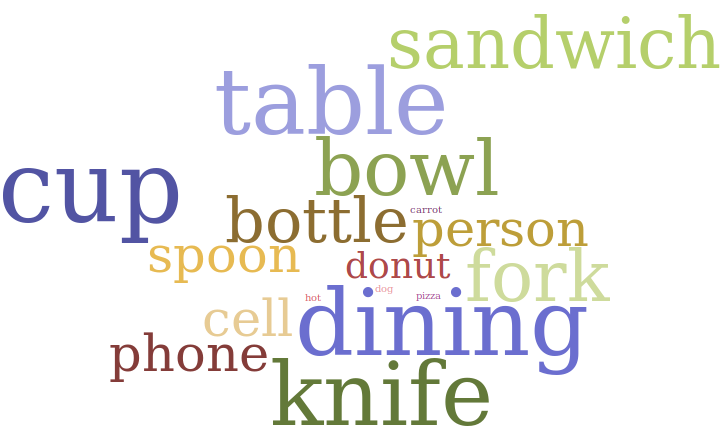
\includegraphics[width=\textwidth]{Sections/4InitialWork/4_images_wordcloud/retina_pic.png}\hfill
      \caption{}
      \end{subfigure}
      \begin{subfigure}{0.3\textwidth}
      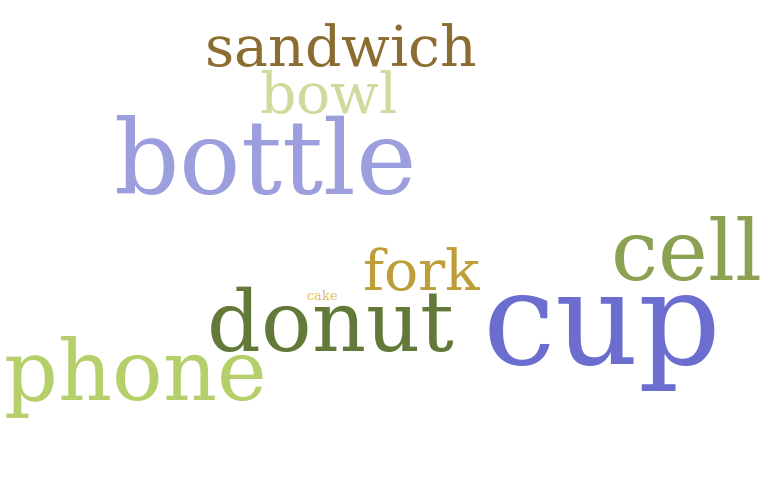
\includegraphics[width=\textwidth]{Sections/4InitialWork/4_images_wordcloud/tiny_yolo_pic.png}\hfill
      \caption{}
      \end{subfigure}
      \caption{Generated Word Clouds; a) Yolo word cloud; b) RetinaNet word cloud; c) TinyYolo word cloud}
    \end{figure}

    \newpage
    
    \begin{itemize}
      \item \textbf{Object Detection Results Analysis}
    \end{itemize}

    

     From the different test runs done in Section \ref{sec:object_test} it is possible to analyse that the TinyYolo model under performs severely compared to RetinaNet and YoloV3. This is expected, as explained in section \ref{sec:tiny_yolo} the TinyYolo model is a smaller model of YOLOv3 that requires less computational resources and that is better suited for more constrained environments with smaller targets.

     Comparing RetinaNet to YoloV3 it is possible to conclude that YoloV3 is more accurate than RetinaNet. For example in the first run, RetinaNet detects knifes and forks in the same place, in third example RetinaNet detects a bus in the place of a building while Yolo is capable of detecting a correctly stop sign that no other model detected.

     As for the word clouds generated in this section, it is possible to notice that in the YoloV3 cloud and the retinaNet cloud there are many more words than the tinyyolo cloud, again, tinyyolo is severely under performing when compared to the other 2 model.
     
     Looking at the Yolo model word cloud its possible to notice some consistency because most of the words have the same size. In the RetinaNet word cloud there are many words from different sizes, this can occur because RetinaNet wrongly detects 1 or 2 object like "pizza", "donut and "person" in one of the images.

     These test runs allow for the conclusion that the YoloV3 model is the better performing one and therefore the one chosen for object detections for the automatic retrieval system. 

\section{Example of a Raw Retrieval System}
\label{sec:alpha_retrieval}

As a first step in building a fully automatic retrieval system an "alpha system" was created without any text processing and very raw on the way it worked. Simply put, a user just needs to write a label, according to one of the words available for detection, and the system will scan all the images that are inside a directory and return the images that have detections of that specific user inputted label. The user is also able to input the minimum percentage probability for the detections, therefore, if the user chooses "cup" and "40\%", objects that are not "cup" or that are "cup" but below the threshold of 40\% wont be returned.

\begin{figure}[H]
  \centering
  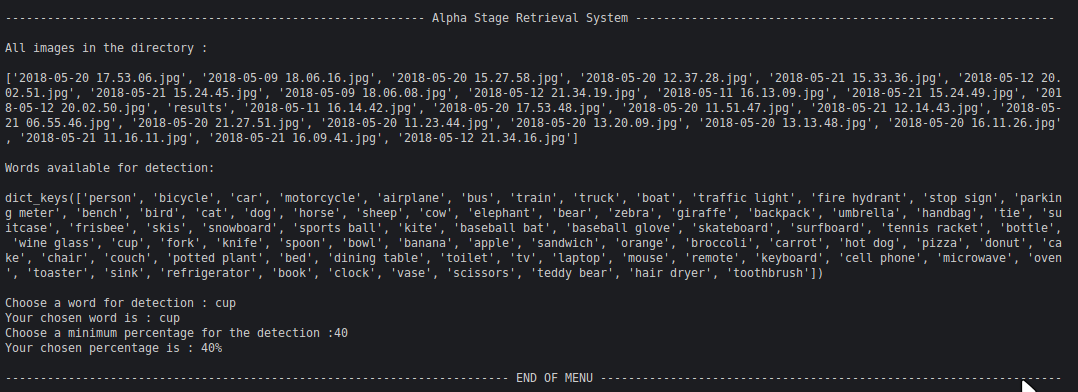
\includegraphics[width = \textwidth]{Sections/4InitialWork/4_images_random/alpha.png}
  \caption{System capable of detecting specific user inputted labels in multiple images. }
  \label{fig:yolov3} 
\end{figure}




\begin{figure}[H]
  \begin{subfigure}{\linewidth}
  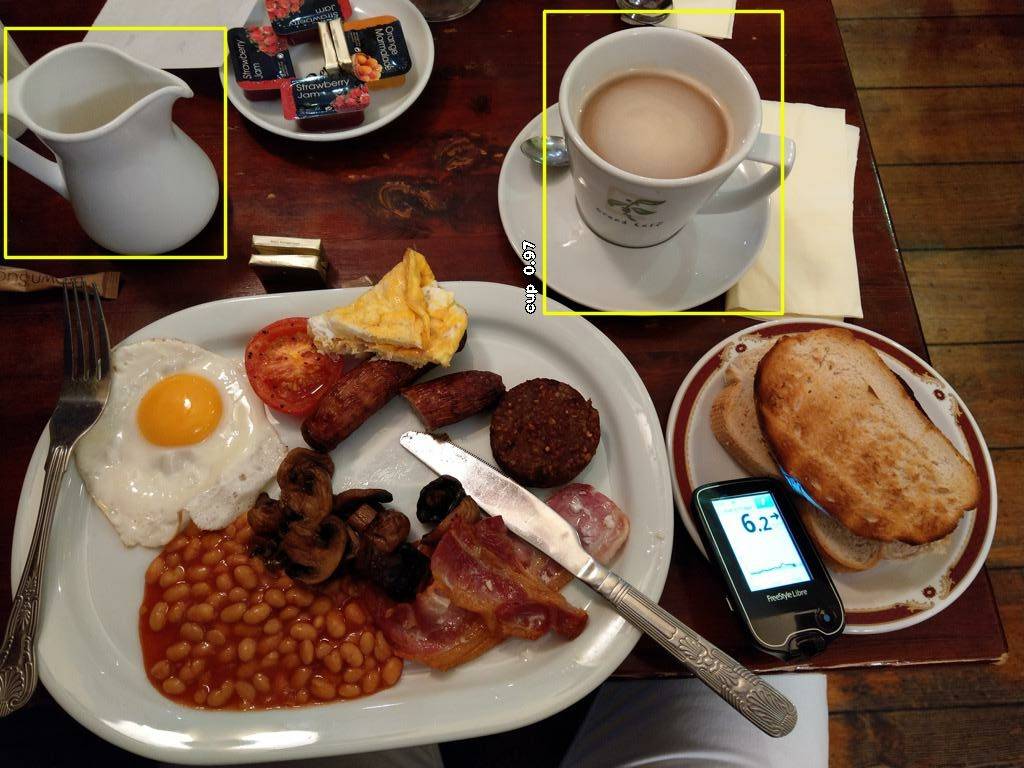
\includegraphics[width=.3\linewidth]{Sections/4InitialWork/4_images_alphasystem/alpha_yolo_2.jpg}\hfill
  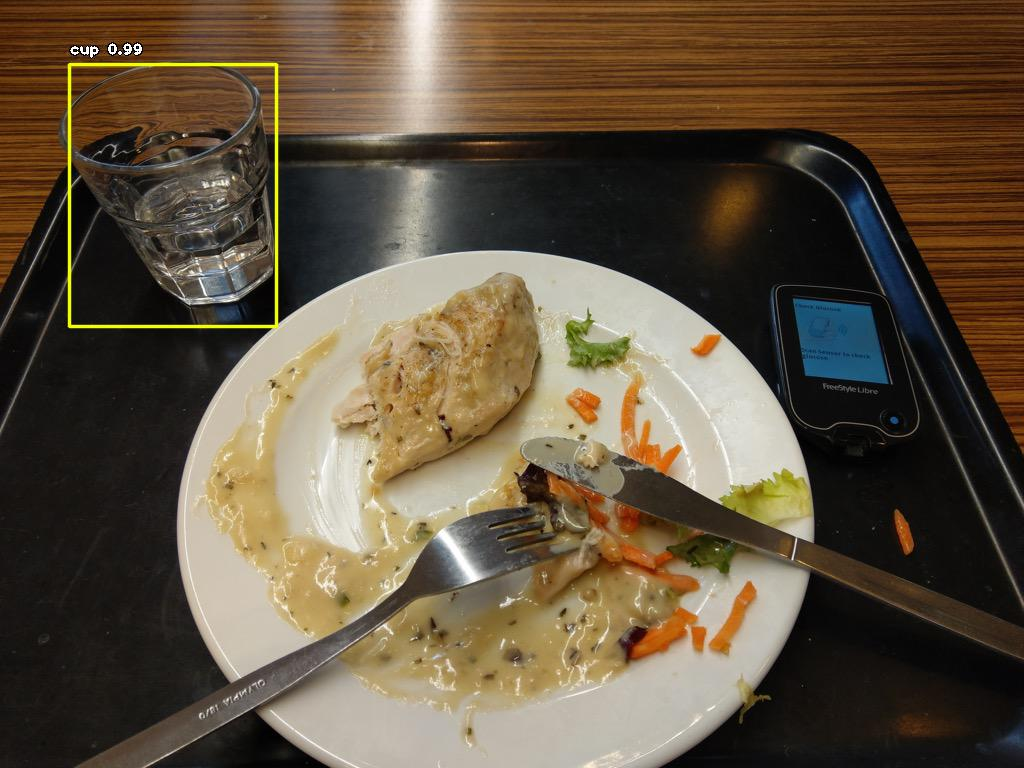
\includegraphics[width=.3\linewidth]{Sections/4InitialWork/4_images_alphasystem/alpha_yolo_3.jpg}\hfill
  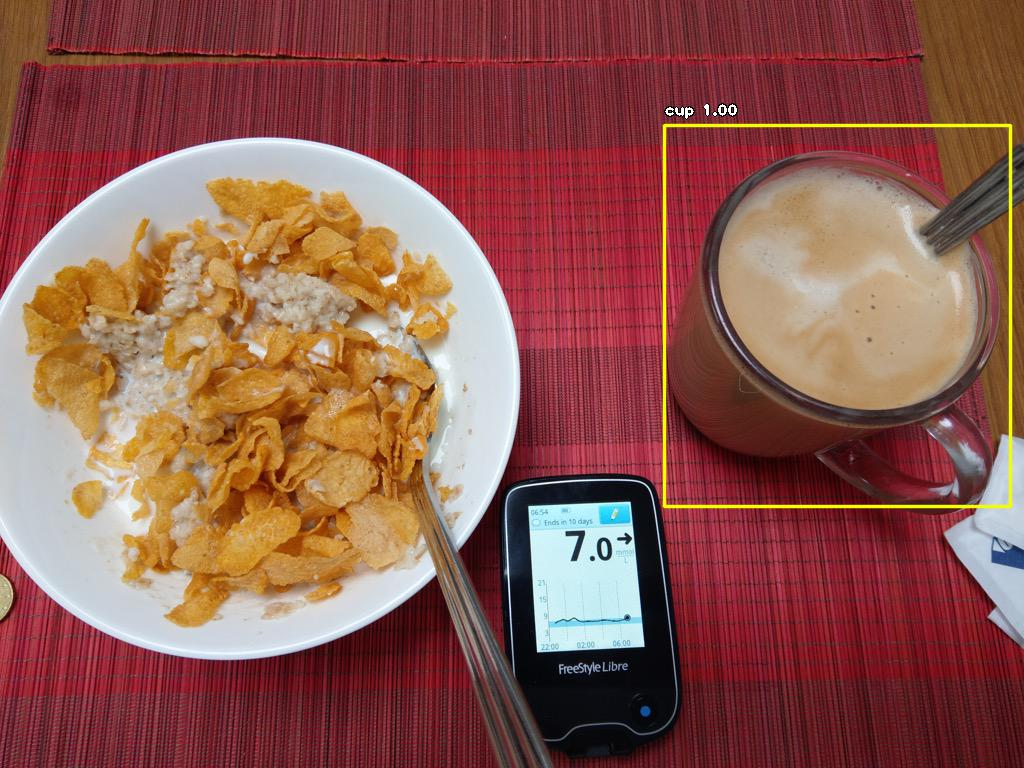
\includegraphics[width=.3\linewidth]{Sections/4InitialWork/4_images_alphasystem/alpha_yolo_4.jpg}
  \end{subfigure}\par\medskip
  \begin{subfigure}{\linewidth}
  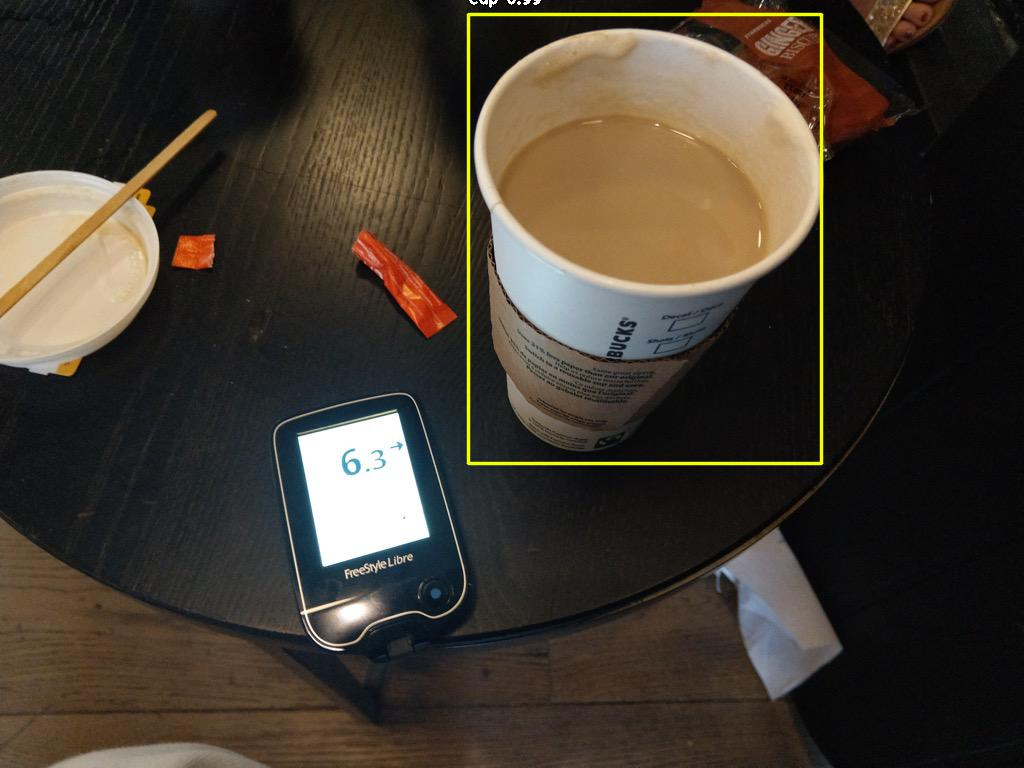
\includegraphics[width=.3\linewidth]{Sections/4InitialWork/4_images_alphasystem/alpha_yolo_5.jpg}\hfill
  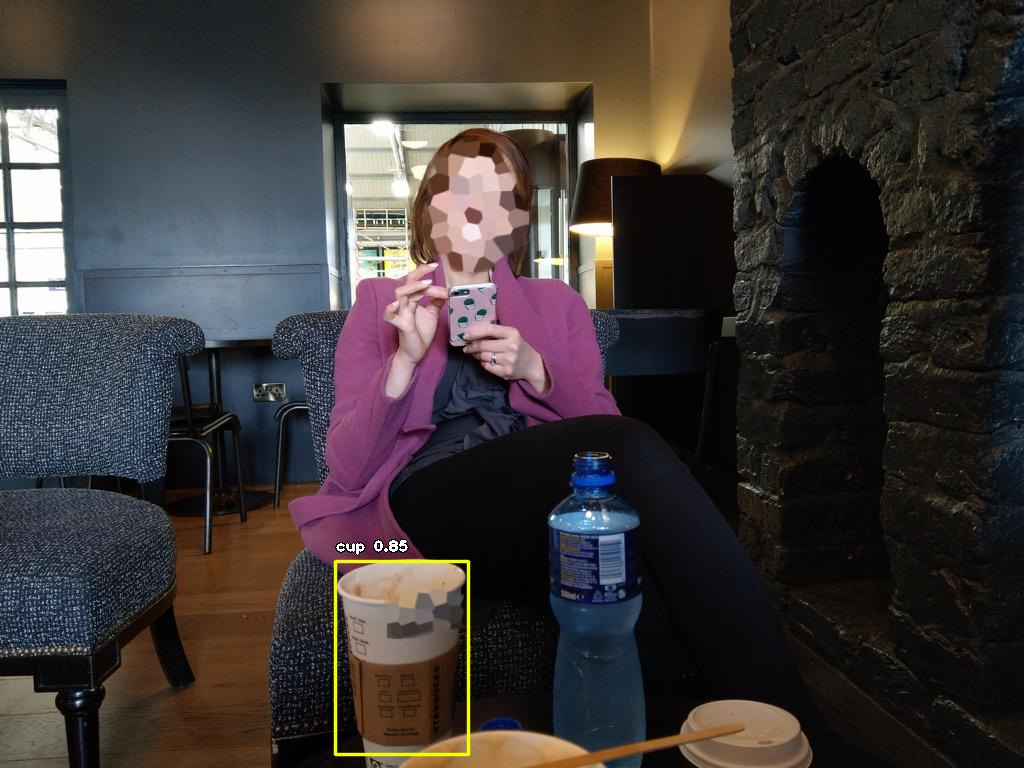
\includegraphics[width=.3\linewidth]{Sections/4InitialWork/4_images_alphasystem/alpha_yolo_6.jpg}\hfill
  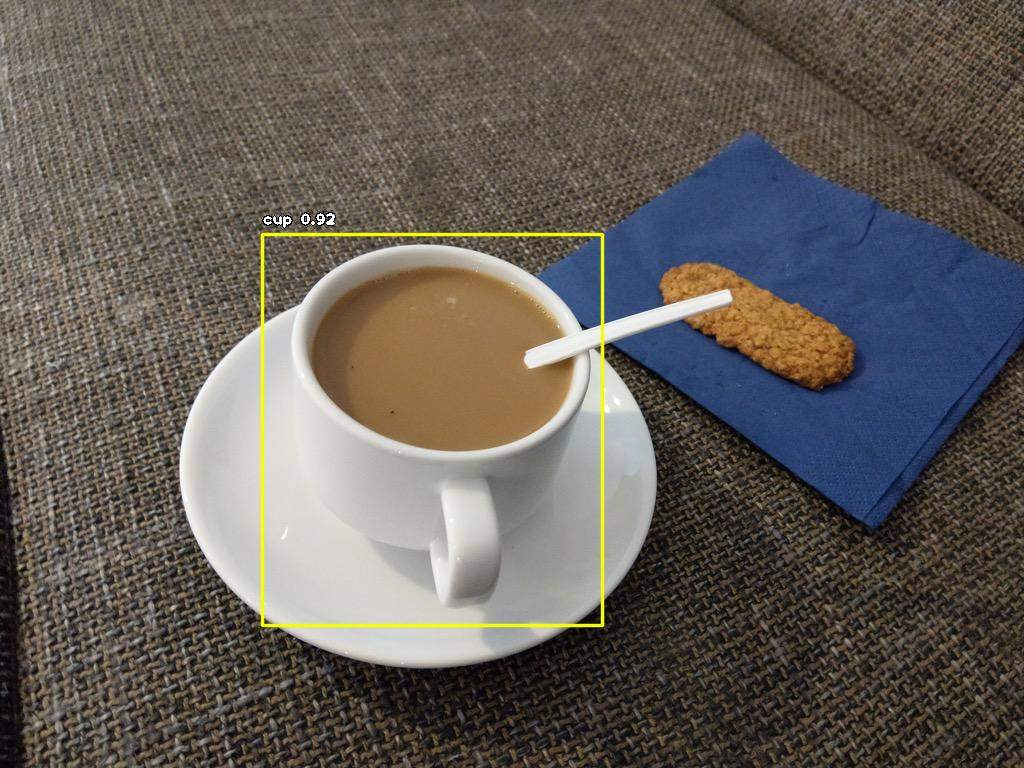
\includegraphics[width=.3\linewidth]{Sections/4InitialWork/4_images_alphasystem/alpha_yolo_7.jpg}
  \end{subfigure}
  \caption{Retrieved images for the label "cup" with "40\%" threshold.}
\end{figure}

\section{Scene Recognition}
\label{sec:scene_recognition}
  In order to detect interiors, exteriors and places a pre-trained model provided by Zhou et al., 2018 \cite{Zhou2018}  trained on the Places365 standard dataset was used. The following example shows the extractions done to a sample picture. 

  \begin{figure}[H]
    \centering
    \captionsetup{justification=centering}

    \begin{subfigure}{0.525\textwidth}
    
    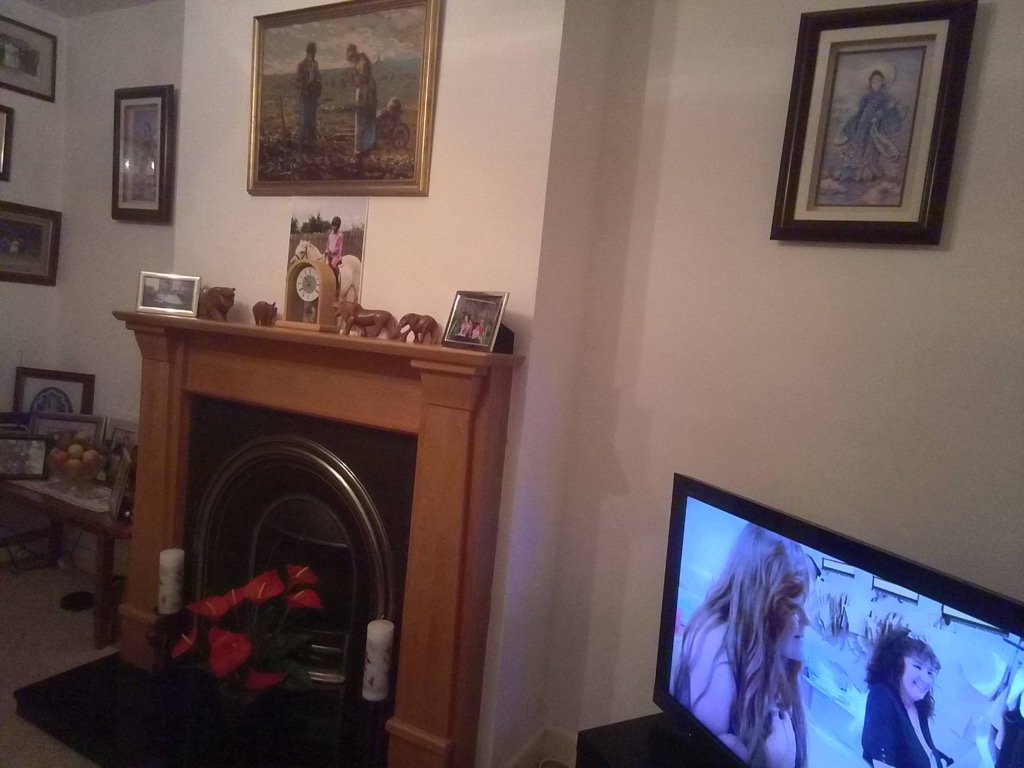
\includegraphics[width=\textwidth]{Sections/4InitialWork/4_images_random/dataset_place.jpg} 
    \caption{}
    \end{subfigure}
    \begin{subfigure}{0.4\textwidth}
    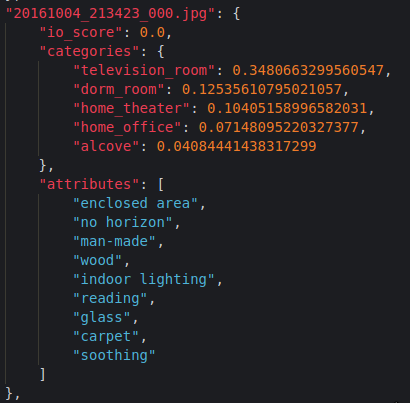
\includegraphics[width=\textwidth]{Sections/4InitialWork/4_images_random/places_detect.png}
    \caption{}
    \end{subfigure}
    
    \caption{Example of a scene recognition; a) Picture 20161004\_213423\_000.jpg from the imageclef dataset; b) Scene recognition model output for that image.}

    \label{fig:imagea}
    \end{figure}


    The "io\_score" represents the interior vs exterior certainty. It ranges from 0 to 1. If its close to 0 it means the image is probably an interior and if it is close to 1 it means it is probably an exterior. In this example, the image is an interior and the "io\_score" is 0, therefore the model predicted correctly that the image is in fact an interior.

    Following up, the "categories" is where the model tries to predict what the image represents in terms of a scene. In this case the model predicts with 34.8\% accuracy that it is a "television\_room" which is also correct, since the image represents a division of a house with a television.

    Finally, the "attributes" is the section where the model tries to describe the picture. Some of the predicaments were "enclosed area", "man-made", "indoor lightning" and so on which are all correct since the image represents a man-made enclosed space structure with indoor-lightning.

\section{Image Processing Submitted Runs Differences}
\label{sec:runs}


    In this year ImageCLEFlifog LMRT subtask, 3 different runs were submitted. The first 2 runs belong to the automatic image retrieval system and the last to the interactive retrieval system. 
    
    Since the interactive system processed the images with detections from a combination of ResNeXt-101 and Feature Pyramid Network architectures in a basic Faster Region-based Convolutional Network (Faster R-CNN) pretrained on the COCO dataset proposed by Mahajan et al. \cite{Mahajan2018} it was decided to reutilize those labels for the automatic system, since the labels were already readily available.  Therefore, for the first submitted run of the automatic image retrieval system it was used the ResNeXt-101 labels and for the second run it was used the YoloV3 \cite{Redmon2018} extracted labels.
    
    The usage of two different set of extracted labels from two different object detection models was mainly done in order to have an understanding if the the difference in labels and the respective scores would help in achieving better results. Furthermore the images were also fully processed with the Places scene recognition model. This exhaustive approach of processing so many images too a  lot of computer processing time and resources


    Figure \ref{fig:image_fully_processed} shows the fully processing of the image shown in Figure \ref{fig:imagea} a) with YoloV3 and PLACES365:
    
    \begin{figure}[H]
      \centering
      \captionsetup{justification=centering}
  
      \begin{subfigure}{0.365\textwidth}
      
      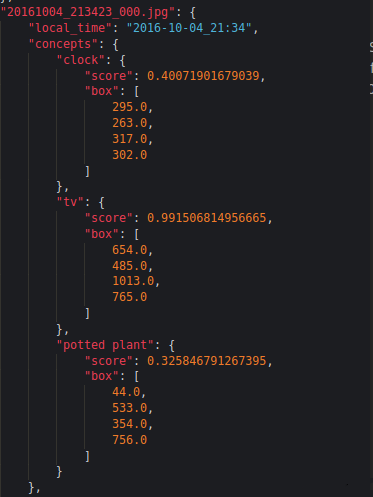
\includegraphics[width=\textwidth]{Sections/4InitialWork/4_images_random/process1.png} 
      \end{subfigure}
      \begin{subfigure}{0.45\textwidth}
      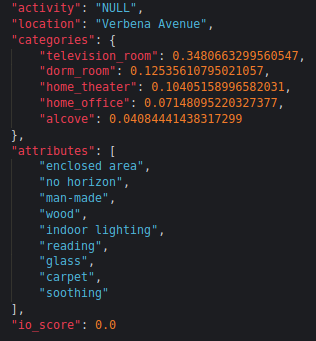
\includegraphics[width=\textwidth]{Sections/4InitialWork/4_images_random/process2.png}
      \end{subfigure}
      \caption{Fully processed image with YOLOv3 and PLACES365.}
      \label{fig:image_fully_processed}
      \end{figure}



      Figure \ref{fig:image_fully_processed_resnext} shows the fully processing of the image shown in Figure \ref{fig:imagea} a) with ResNeXt-101 and PLACES365:
       
    \begin{figure}[H]
      \centering
      \captionsetup{justification=centering}
  
      \begin{subfigure}{0.3\textwidth}
      
      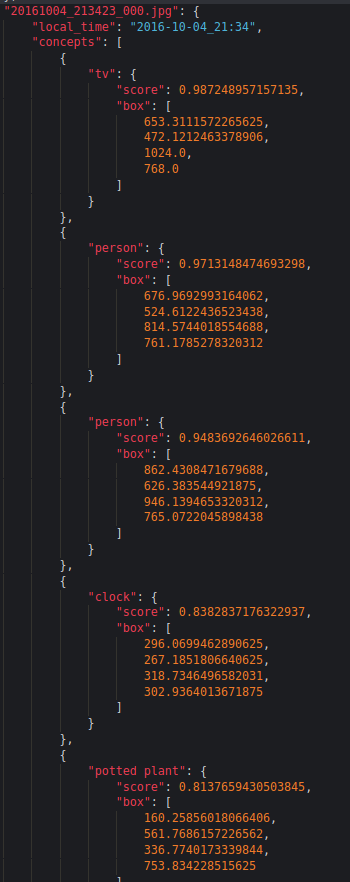
\includegraphics[width=\textwidth]{Sections/4InitialWork/4_images_random/res1.png} 
      \end{subfigure}
      \begin{subfigure}{0.3\textwidth}
      \includegraphics[width=\textwidth]{Sections/4InitialWork/4_images_random/res2.png}
      \end{subfigure}
      \begin{subfigure}{0.3\textwidth}
        \includegraphics[width=\textwidth]{Sections/4InitialWork/4_images_random/res3.png}
        \end{subfigure}
      \caption{Fully processed image with ResNeXt-101 and PLACES365.}
      \label{fig:image_fully_processed_resnext}
      \end{figure}


      The "activity" and "location" were extracted from the data provided by the organizers in a .csv file. However,  that data is not accurate enough, and a good option would be to use activity recognition algorithms to extract activities from images. Furthermore, the processing time was already to high with the current setup.
      The "local\_time" was extracted directly from the picture name.
      The "box" is the location of the given "concept" in the image according to the pixels of the image.



\newpage
\section{Text Word Extraction and Categorization}
\label{sec:text}

In the text mining/processing stage, the query topics are analysed using Natural Language Processing tools to extract relevant words in order to retrieve the desired moment. Those words are compared with the visual concepts words obtained in the image processing stage. 

The SpaCy en\_core\_web\_md model \cite{Spacy2017} is used to analyse the query topics fully, extracting relevant words from the title, the description and narrative. This model is an english multi-task CNN trained on OntoNotes, with GloVe vectors trained on Common Crawl and is a general-purpose pretrained model to predict named entities, part-of-speech tags and syntactic dependencies. It can be used out-of-the-box and fine-tuned on more specific data \cite{Spacy2017}. This model was chosen since it is specific for the English language and it is medium sized (48 MB) which is a good balance between loading speed and accuracy. The larger SpaCy model is 756 MB (79 times larger) which makes it much more slower to load and process. However, the difference in performance between the two models for the given task is negligibly.




The words extracted are divided into 10 categories being them : "relevant things", "activities", "dates", "locations", "inside", "outside", "negative relevant things", "negative activities", "negative locations" and "negative dates". The importance of this extraction and categorization is done in order to later compare this extracted textual data with the extracted visual data from all of the images. To give a clear example, having the sentence from Figure \ref{fig:spacy_labels} it is crucial to correctly extract the concept "fast food" and categorize it in the "relevant things" textual category in order to compare with the "concepts" visual category. It is also important to extract the word "airport" and categorize it in the "locations" category in order to compare with the "location" visual category. It would not make sense toe extract the word "fast food" and categorize it in the "locations" textual category for later comparing with the "location" visual category.

In order to assign words to each category some linguistic rules were defined,
such as semantic and syntactic rules. Semantic rules build the meaning of the
sentence from its words and how words combine syntactically. Syntax rules refer to
the rules that govern the ways in which words combine to form phrases and
sentences. 

\begin{figure}[H]
    \centering
    \captionsetup{justification=centering}
    \includegraphics[width =  \textwidth]{Sections/6textprocessing/images/spacy.png}
    \caption{Linguistic annotations generated by the SpaCy library \cite{Spacy2017} for the narrative of the topic 6 of the test topics.}
    \label{fig:spacy_labels}
  \end{figure}

 
Using Figure \ref{fig:spacy_labels} to illustrate, the extracted words for the the narrative of the test topic 6 are presented next:
\newpage
    \begin{itemize}
      \itemsep0em
        \item \textbf{relevant things} : "fast food".
        \item \textbf{activities} : "ordering", "ordering fast food".
        \item \textbf{locations} : "airport".
        \item \textbf{inside} : "True".
        \item \textbf{outside}: "False".
       
    \end{itemize}

  \subsection{Implemented Syntax Rules}
  The syntax rules were created from a continuous work from last year \cite{Ribeiro2019}. However, this year many more rules were implemented and more categories for word categorization were created like the negatives category. Something very important to note is that the syntax from the dev topics and test topics is very specific and very similar, therefore some syntax rules that were created probably wouldn't work so well for other kinds of documents with different syntaxes.

  An excerpt of few of the most simple syntax rules that were applied to the extraction and categorization of the textual data are presented next:
  
  \begin{itemize}
    
      \item  If the word is a "VERB" and ends with "ing", like "ordering" then it probably is an activity and if the words that follows are "NOUN" then those words probably refer to a location or an object. 
      
      
      \item  If the word is and "ADP" (adposition) and its either "in" or "at" then the words that follow are probably locations and usually means that the moment occurs inside a location and not outside, the category "inside" is then flagged to "True" and "outside" is flagged to "False".
      
      \item If the word is a "NUM" (number) then it probably refers to a year.
      
      \item If the word isSpaCy en\_core\_web\_md a "VERB", and the following word is a "poss" (possession modifier) and if the following word to the last is a "NOUN", then all of this sentence referes to an activity and the NOUN to an object. For example "Repairing his car". "Repairing" and "Repairing his car" are the activities and "car" is the relevant thing.
      
      \item If the sentence has an auxiliary verb, the main verb usually corresponds to an activity and the words that follow the main verb may be objects or locations.
      
      \item If the word is an "ADJ" (adjective) then the following word is probably an object. It can also be a bi-gram like "ice cream" or in this case "fast food".
      
      \item If the sentence ends with "not considered relevant" the extracted words go to the negative categories.
      
      \item Rules for the extraction of dates, like the day of the week, the month or even years were also created. However do the the syntax of the test topics, since they had no reference to dates in the text, the dates category was discarded in order to save time. Nevertheless, for the dev topics dates were used and produced good results. As an example if in the topic it was said that the moment happened on a "wednesday" or in year 2014, only pictures from wednesday or the year 2014 were retrieved.

    \end{itemize}
      
    

    
    
    The main idea in creating these syntax rules was to look at the linguistic annotations that the SpaCy model provided and see which words were the ones important for extraction. This was something that was complex to do, but after making the algorithm work for the dev topics, the test topics did not require much iteration since the syntax was very much identical to the dev topics. However, the word extraction and categorization is not flawless and sometimes it places things to wrong categories or misses one or two words for extraction. However, in the current state, it can be considered that it it working well enough. 
        
    Furthermore, many more syntax rules were implemented which made the algorithm very complex.
  



\section{Image Retrieval}
\label{sec:retrieval}

    In the retrieval step the images are recovered according to the desired query topic.
    As an example Figure \ref{fig:testtopic} represents the test topic number 7.
   
    \begin{figure}[H]
        \centering
        \captionsetup{justification=centering}
        \includegraphics[width = \textwidth]{Sections/6textprocessing/images/topic.png}
        \caption{Test topic number 7.}
        \label{fig:testtopic}
      \end{figure}
      
      The extracted words of the title, description and narrative are as follows:

      \begin{itemize}
        \itemsep0em
        \item \textbf{relevant things} : 
            "seafood",
            "parts",
            "shrimp",
            "lobster",
            "salmon".
        \item \textbf{activities} : "eating",
        "eating seafood"
        \item \textbf{locations} : "restaurant",  "evening time".
        \item \textbf{inside} : "True".
        \item \textbf{outside}: "False".
        \item \textbf{dates}: NULL.
        \item \textbf{negative relevant thing}: NULL.
        \item \textbf{negative activities}: NULL.
        \item \textbf{negative locations}:  NULL.
        \item \textbf{negative dates}: NULL.
       
    \end{itemize}
\newpage
    An important detail to be noticed is that the extracted words "evening time" are wrongly categorized on the "locations" textual category. The main reason for this error to occur is probably a direct consequence of one of the syntax rules that did not work as intended for this specific case. The sentence is written in the following manner "The moments show u1 was eating seafood in any restaurant in the evening time.." and one of the rules for locations extraction is, as previously discussed, if the word is an "ADP" (adposition) and its either "in" or "at" then the words that follow are probably locations. However, in this case, there are two different "in", one refers to "restaurant" which is a location and the other to "evening time" which is not a location. This is an example of the algorithm not working as intended.

    \subsection{Retrieving Images According to the Similarity Between Words}

    In order to retrieve images according to a defined moment in a textual topic a comparison is made between the extracted labels from the images and the words extracted from the topics. This comparison is done trough the calculation of similarity score obtained by an NLP model provided by the SpaCy library. This similarity score alongside the weight attributed to each category is critical for the calculation of the confidence score for each image. The images with the highest confidence scores for a given topic are selected for retrieval.
    
    

    \begin{itemize}
      \item \textbf{Similarity Score Computation}
    \end{itemize}

    The SpaCy en\_core\_web\_md model allows the computer to calculate the similarity between the visual concepts and the extracted data. As an example of similarity between words using the described model, the word "television" and "seafood" have a similarity of approximately 0.07 (7\%) while "television" and "screen" have a similarity of approximately 0.43 (43\%).
    
      
    Using Figures \ref{fig:image_fully_processed} and \ref{fig:image_fully_processed_resnext} to illustrate the different categories, the calculation of the similarity scores is done trough the comparison of the extracted words and the visual concepts:
    \begin{enumerate}
        \itemsep0em
        \item The visual category "concepts" is compared to the textual category "relevant things";
        \item The visual category "concepts" is compared to the textual category "negative relevant things";
        \item The visual category "activity" is compared to the textual category "activities";
        \item The visual category "activity" is compared to the textual category "negative activities";
        \item The visual category "location" is compared to the textual category "locations";
        \item The visual category "location" is compared to the textual category "negative locations";
        \item "Depending if the textual category "inside" = "True" / "False" the visual category "io\_score" value will have different impact on the confidence score.
    \end{enumerate}

    \begin{itemize}
      \item \textbf{Category Weight}
    \end{itemize}


    The weight for each category is obtained through two different factors, an importance weight factor and a distributed weight factor. The weight of the category is therefore the sum of the importance weight factor and the distributed weight factor. 

    \begin{align*}
      &\textbf{Weight}  =   ImportanceFactor + DistributedFactor \\ 
  \end{align*}

    
    \begin{itemize}
      \item \textbf{Importance Weight Factor}
    \end{itemize}

    The importance weight factor is a value that is assigned to the positive available categories that are not empty. It is a pre-defined valor and is the factor that gives more importance to one category than others to the contribution of the confidence score computation. This factor ranges from 0 to 1 and the sum of all of the factors is equal to 1. For example, if the category of "relevant things" is worth 0.4 and if the category of "activities" is worth 0.2, then "relevant things" has a weight always two times higher than "activities" for the computation of the confidence score.

    \begin{itemize}
      \item \textbf{Distributed Weight Factor}
    \end{itemize}

    The distributed weight factor is the distribution of the importance weight factor from an empty category to all other categories that are not empty. To make it clear, if the text mining algorithm didn't extract any words to the "activities" category then there is no use in calculating millions of similarity scores that are comparing the images category "activities" with the NULL "activities" textual category . 

        
   Assuming the following example:
   \begin{enumerate}
    \item (Not Empty category) "Relevant Things" importance weight factor = 0.4 (40\%);
    \item (Empty category)"Activities" importance weight factor =  0.2 (20\%);
    \item (Not Empty category) "Inside/Outside" importance weight factor = 0.3 (30\%);
    \item (Not Empty category) "Location" importance weight factor = 0.1 (10\%);
    \item Sum of all importance factors = 1.
   \end{enumerate}

   In this example, the "Relevant Things" category is worth 40\% of the sum of all importance factors while "Activities" is worth 20\%, "Inside/Outside" is worth 30\% and "Location" is worth 10\%. Therefore, if by any means the "Activities" category is empty, the importance weight factor of this category will be distributed to all other categories in the following way:

   \begin{enumerate}
    \item Distribution : 4x + 3x + x = 0.2 (=) x = 0.25;
    \item Weight "Relevant Things" = 0.4 + 4*0.25 = 0.5 (50\%);
    \item Weight "Activities" = 0;
    \item Weight "Inside/Outside" category = 0.3 + 3*0.25 = 0.375 (37.5\%);
    \item Weight "Location" =  0.1 + 0.25 = 0.125 (12.5\%);
    \item Sum of all weights = 1.
   \end{enumerate}


   This distribution achieves two important things, the sum of all weights is always 1 (100\%) and the ratio between categories is always the same. In the begin "Relevant things" was 40\% and "Location" was 10\%  which is a ratio of 4 and in the end "Relevant things" is 50\% and "Location" is 12.5\% which is still a ratio of 4. This means that in this situation "Relevant things" has a weight of 50\% for the computation of the confidence score.
   
   The negative categories works the same way, but instead of contributing for the confidence score, it decreases the value.

    

    \begin{itemize}
      \item \textbf{Confidence Score Computation}
    \end{itemize}

    The confidence score is a value that also ranges from 0 to 1 (0\% to 100\%) and is the final value that gives the verdict on how an image relates to a given moment. A score of 20\% means that the image is not related while a higher score of 80\% means that an image probably relates to the moment. 

    The computation of the confidence score is also influenced by the score of the image concepts obtained trough the image processing phase. This means that an image with low prediction score (from the image processing stage) will have a lower confidence score. 

    Since the images dataset consists in 200.000 images and the test topic dataset consists on 10 topics, approximately 2.000.000 confidence score calculations had to be computed. This step is extremely exhaustive on computer time and resources, which made it hard to make adjustments, correct errors and bugs in the code.
        
   


    In order to have a better visualization of how all of this calculations are done the follow equations illustrate all the steps needed in order to compute the confidence:

    \begin{align*}
        &\textbf{ConceptScore}  =   [Weight_1]\times[HighestSimilarityScore]\times[VisualScore] \\ 
        &\textbf{LocationScore} = [Weight_2]\times[HighestSimilarityScore] \\ 
      &\textbf{ActivityScore} =  [Weight_3]\times[HighestSimilarityScore]\\
        &\textbf{InsideScore}   =  [Weight_4]\times(1-[ioscore])\\
        &\textbf{OutsideScore}  =  [Weight_5]\times([ioscore])\\
        &\textbf{PositiveScore}  =  ConceptScore + LocationScore + ActivityScore + (Inside||Ouside)Score\\
        &\textbf{NegativeConceptScore}  =  [Weight_6]\times[HighestSimilarityScore]\times[VisualScore]\\
        &\textbf{NegativeLocationScore}  =  [Weight_7]\times[HighestSimilarityScore]\\
        &\textbf{NegativeActivityScore}  =  [Weight_8]\times[HighestSimilarityScore]\\
        &\textbf{NegativeScore}  =  Negative(ConceptScore + LocationScore + ActivityScore) \\
        &\textbf{ConfidenceScore}  =  PositiveScore - NegativeScore\\
  \end{align*}
  

  \begin{itemize}
    \item \textbf{Image Retrieval}
  \end{itemize}

    Finally, a script runs through all the selected confidence scores for a given
    query topic and stores the 50 pictures with the highest confidence score for each topic. The 10 highest pictures for each topic are the ones who count for the f1@measure score.
       
    \begin{itemize}
      \item \textbf{Discarded Categories}
    \end{itemize}
    
    Due to the fact that the PLACES365 scene recognition model extracts scenes with very low scores, rarely above 30\%-40\% it was decided to discard the category "categories" and "attributes" from contributing to the confidence score in order to save processing time.

   \newpage
    \begin{itemize}
      \item \textbf{General Thresholds}
    \end{itemize}

    A few general thresholds were defined:

   \begin{enumerate}
    \item Visual concept label score minimum threshold : 0.3;
    \item "Relevant Things" category score  minimum threshold: 0.15;
    \item Confidence score minimum threshold  : 0.25;
   \end{enumerate}


   The thresholds were implemented through some trial and error during the test phases, and it merely serves the purpose of saving some computational time so that confidence scores of images with low scores are not fully processed. 



    \section{Submitted Run 1}
      \label{sec:run1}

    The first run to be submitted for the imageclef LMRT subtask used a combination of ResNeXt-101 and Feature Pyramid Network architectures in a basic Faster Region-based Convolutional Network (Faster R-CNN) pretrained on the COCO dataset for the extraction of visual concepts.

    In this run all of the importance weight factors for all categories were the same. This means that each category counts the same for the computation of the confidence score. No category is more important or less important. When a category is empty, their respective importance factor is equally apportionated to all other categories but never to the negative categories. If a negative category importance factor is negative, their factor is apportionated to the other negative categories. And if a positive category is empty, their factor is apportionated to the positive categories.

    Another aspect of Run 1 is that the negative categories can only impact the confidence score up to 0.5.
    
 

    \section{Submitted Run 2}
    \label{sec:run2}
    
    In the second run, the object detection algorithm used is the YoloV3 model pretrained in the COCO dataset.  It was decided to define the importance weight factor differently for each category. It was given a bigger importance to specific categories like "relevant things" and "ioscore". Categories like ”activities” and ”locations” get a lesser importance weight factor since they are being compared to the organizers label data which is limiting and lesser accurate.  Another difference from Run 1 to Run 2 is that all of the negative categories were discarded from contributing to the confidence score, in order to save processing time and since the first results from Run 1 did not appear to impact much.
    
